\documentclass[10pt]{article}
\usepackage[utf8]{inputenc}
\usepackage[english]{babel}
\usepackage[font=small,labelfont=bf]{caption}
\usepackage{geometry}
\usepackage{natbib}
\usepackage{pxfonts}
\usepackage{graphicx}
% \graphicspath{ {./figures-low/} }
% \DeclareGraphicsExtensions{.png,.pdf}
\graphicspath{ {./figures-default/} }
\usepackage{newfloat}
\usepackage{setspace}
\usepackage{hyperref}
\usepackage{lineno}
\usepackage{placeins}
\usepackage{authblk}
\usepackage{textcomp}
\usepackage{listings}
\bibliographystyle{apalike}

\doublespacing
\linenumbers

\title{\Large The psychological arrow of time drives temporal asymmetries in inferring unobserved past and future events}
\author[1]{Xinming Xu}
\author[2]{Ziyan Zhu}
\author[3]{Xueyao Zheng}
\author[1, $\star$]{Jeremy R. Manning}
\affil[1]{Dartmouth College, Hanover, NH, USA}
\affil[2]{Peking University, Beijing, China}
\affil[3]{University of California at Davis, CA, USA}
\affil[$\star$]{Address correspondence to jeremy.r.manning@dartmouth.edu}

% tables
\newcommand{\stimDescription}{S1}
\newcommand{\metaTable}{S2}

% figures
\newcommand{\segments}{S1}
\newcommand{\events}{S2}
\newcommand{\references}{S3}
\newcommand{\MethodsReplExp}{S4}
\newcommand{\targetAsymmetries}{S5}
\newcommand{\hitRates}{S6}
\newcommand{\characterRefs}{S7}
\newcommand{\refAdjacent}{S8}
\newcommand{\referringReferenced}{S9}



\begin{document}

\maketitle

\begin{abstract} {\footnotesize{ How much can we infer about the past and
future, given our knowledge of the present? Unlike temporally symmetric
inferences about simple sequences, inferences about our own lives are
asymmetric: we are better able to infer the past than the future, since we
remember our past but not our future (i.e., the psychological arrow of time).
What happens when both the past and future are unobserved, as when we make
inferences about \textit{other} people's lives? We had participants in two
experiments view segments of two character-driven television dramas. They wrote
out what would happen just before or after each just-watched segment.
Participants were better at inferring past (versus future) events. This
asymmetry was driven by participants’ reliance on characters’ conversational
references in the narrative, which tended to favor the past. We also carried
out a meta analysis to estimate the prevalence of these asymmetries in hundreds
of millions of dialogues from television shows, popular movies, novels, and
written and spoken natural conversations. We found that, on average, references
to the past are roughly 1.5--2 times more prevalent than references to the
future. Our work reveals a temporal asymmetry in how observations of other
people’s behaviors can inform us about the past and future.

\textbf{Keywords: arrow of time, prediction, retrodiction, narrative, conversation}}}

\end{abstract}

\section*{Introduction} 

What we experience in the current moment tells us about \textit{now}-- but what
does it tell us about the past or future? And does the current moment tell us,
as human observers, \textit{more} about the past or about the future? One way
of examining these questions is to consider highly simplified scenarios that
are artificially constructed in the laboratory \citep[e.g., ][]{MaheEtal22}. At
one extreme, for deterministic sequences with \textit{known} rules, knowing the
current state provides the observer with sufficient information to exactly
reconstruct the entire past and future history of the stimulus. At another
extreme, for purely random sequences, observing the current state provides no
information about the past \textit{or} future.

Sequences generated by stochastic processes fall somewhere between these two
extremes. For Markov processes, where each state is solely dependent on the
immediately preceding state, Shannon entropy may be used to quantify the
uncertainty of the past and future states, given the present state.
\cite{Cove94} showed that, for any stationary process (i.e., processes in
equilibrium), Markov or otherwise, the present state provides equal information
(i.e., mutual information) about past and future states~\citep[also
see][]{BialEtal01, ElliEtal09}. Further, there is some evidence that humans are
similarly adept at inferring the most likely previous and next items in
sequences governed by stochastic Markov processes~\citep{JonePash07}.

Deterministic, random, and probabilistic sequences (in equilibrium) are all
symmetric: the present state of these sequences is equally informative about
past versus future states. In contrast, our subjective experience in everyday
life is that we know more about our own past than our
future~\citep[e.g.,][]{Horw87}. We have memories of our past that we carry with
us into the present moment, but we do not have memories of our
yet-to-be-experienced future. This temporal asymmetry imposes an ``arrow of
time'' on our subjective experience, known as the \textit{psychological arrow
of time}~\citep[e.g.,][]{Hawk85}.

\begin{figure}[tp]
  \centering
  \includegraphics[width=\textwidth]{intro1}

  \caption{\textbf{Retrodiction, retrospection, and prediction.} In one's own
  life, one may draw on memory to retrospect (i.e., review or re-evaluate) the
  past or predict the future. This process is time-asymmetric, since our own
  past is (typically) observed whereas our future is not. When we make
  inferences about \textit{other} people's lives, however, we often have
  uncertainty about both their past and future, since we may have observed
  neither. We may \textit{retrodict} the unobserved past and predict the
  unobserved future of other people's lives.}

  \label{fig:intro1}
\end{figure}

Although the psychological arrow of time implies that we should be better able
to infer our past than our future, how generally does this temporal asymmetry
hold? And does the asymmetry hold only for our own experiences (due to our
memories), or is the asymmetry a general property of any real-life event
sequence? In real-world situations (and narratives) where we are
\textit{equally} ignorant of the past and future, as for \textit{other}
people's lives where we lack memories of the relevant past, are our inferences
about the past and future symmetric or asymmetric? For example, imagine that
you are meeting a stranger for the first time. At the moment of your meeting,
you lack both memories of their past and knowledge about what they might do in
the future. After your first encounter with the stranger, would you be able to
more accurately or easily form inferences about what had happened in their past
(\textit{retrodiction}) or what will happen in their future
(\textit{prediction}; Fig.~\ref{fig:intro1})? Or suppose you started watching a
movie partway through. Again, you would enter the moment of watching without
memories of prior parts of the movie. Given your observations in the present,
would your guesses about what had happened before you started watching be more
(or less) accurate than your guesses about what will happen next? In general,
when the past and future are \textit{both} unobserved, are we better at
inferring the past or the future in real-world settings? Narrative stimuli,
such as stories and movies, can provide a useful testbed for exploring several
of these questions.

Although narratives are unlikely to be confused with one's own experiences,
narratives mirror some of the structure of real-world experiences. Character
behaviors and interactions are often designed in a way that helps the audience
connect with or relate to the characters. Events in narratives also unfold in
ways that are intended to build rapport or engagement with the audience. This
might be accomplished by having events follow a believable structure that is
reminiscent of real-world experiences, or by designing the audience's
experiences in ways that communicate clear ``rules'' or ``features'' that help
to immerse the audience in the narrative's universe. The characters in a
realistic narrative can also be written to behave in ways reminiscent of
real-world people. These same aspects of narratives that authors use to drive
engagement with events and characters can lead narratives to replicate some
core aspects of real-world experiences that are typically lost or overlooked in
traditional sequence learning paradigms. Narratives can drive the audience to
build situation models~\citep{RadvCope06, ZwaaRadv98} of the narrative's
universe, or to form a theory of mind of and make predictions about the
characters~\citep{TamiThor18, KostSaxe13}. Events in narratives may unfold in a
consistent or logical way, but they also exhibit complex and meaningful
interactions across events reminiscent of real-world experiences (but not
necessarily the simple sequences traditionally used in the statistical learning
literature).

One key difference between simple artificial sequences and more naturalistic
(real or narrative) sequences is that naturalistic sequences often incorporate
other people. Despite the past and future being equally unknown to \textit{the
observer} prior to the current moment, other people, and realistic characters
in narratives, have their own psychological arrows of time. Specifically, they
have memories of their own pasts. Other people's asymmetric knowledge about
their \textit{own} pasts and futures might affect their behaviors (e.g.,
conversations). In turn, this might provide time-asymmetric clues that favor
the past~\citep[e.g., other people might talk more about their own pasts than
their futures; ][]{DemiEtal18}. If observers leverage these clues from other
people's asymmetric knowledge, then observers should also be better at
inferring the past (versus the future) of other people's lives. Alternatively,
inferences about other people's lives may be more like inferences about
artificial statistical sequences~\citep[e.g., perhaps solely relying on
statistical regularities like event schemas, scripts, or situation
models][]{RadvCope06, ZwaaRadv98, BoweEtal79, RangRitc12, BaldEtal18}. If so,
then the accuracy of inferences about the past and the future of others' lives
should be approximately equal. We note that the aforementioned authors make no
specific claims about temporal symmetries or asymmetries. Rather, we claim that
statistical regularities might \textit{imply} symmetry (e.g., if you are on
step $n$ of an unfolding schema, this suggests you have just completed step $n
- 1$ and that you are next likely to encounter step $n + 1$).

We designed a naturalistic paradigm for exposing participants to scenarios
where the past and future were equally unobserved. We asked our participants to
watch a series of movie segments drawn from a character-driven dramatic
television show. Across the conditions and trials in the experiment,
participants made free-form text responses to either retrodict what had
happened in the previous segment, predict what would happen in the next
segment, or recall what happened in the just-watched segment. We used manual
annotations and sentence-level natural language processing models to
characterize participants' responses. To foreshadow our results, we found that
participants were overall better at retrodicting the past than predicting the
future. This appeared to be driven by two main factors. First, characters more
often referred to past events than future (e.g., planned) events, and this
influenced participants' responses. Second, associations and dependencies
between temporally adjacent events enabled participants to form estimates about
nearby events (e.g., to a just-watched scene or a past or future event
referenced in an observed conversation). We also ran a pre-registered
replication study to confirm that these findings generalized to another
television show and group of participants. Finally, we ran a meta analysis
using natural language processing to estimate the prevelance of references to
past and future events in hundreds of millions of dialogues drawn from
television shows, popular movies, novels, and written and spoken natural
conversations. Taken together, our work reveals a temporal asymmetry in how
observations of other humans’ behaviors inform us about the past versus the
future.

\section*{Results}

Participants in our main experiment ($n = 36$) watched segments from two
storylines, drawn from the CBS television show \textit{Why Women Kill}. Each
storyline comprised 11 segments (mean duration: 2.05~min; range:
0.97--3.87~min, Table~\stimDescription). We asked participants to use free-form
(typed) text responses to retrodict what had happened prior to a just-watched
segment, predict what would happen next, or recall what they had just watched
(Fig.~\ref{fig:method}, \textit{Task design}). We referred to the
to-be-retrodicted, to-be-predicted, or to-be-recalled segment as the
\textit{target segment} for each response. We systematically varied whether
participants watched the segments in forward or reverse chronological order,
and how many segments they had seen prior to making a response (see
\textit{Methods}).

\begin{figure}[tp]
  \centering
  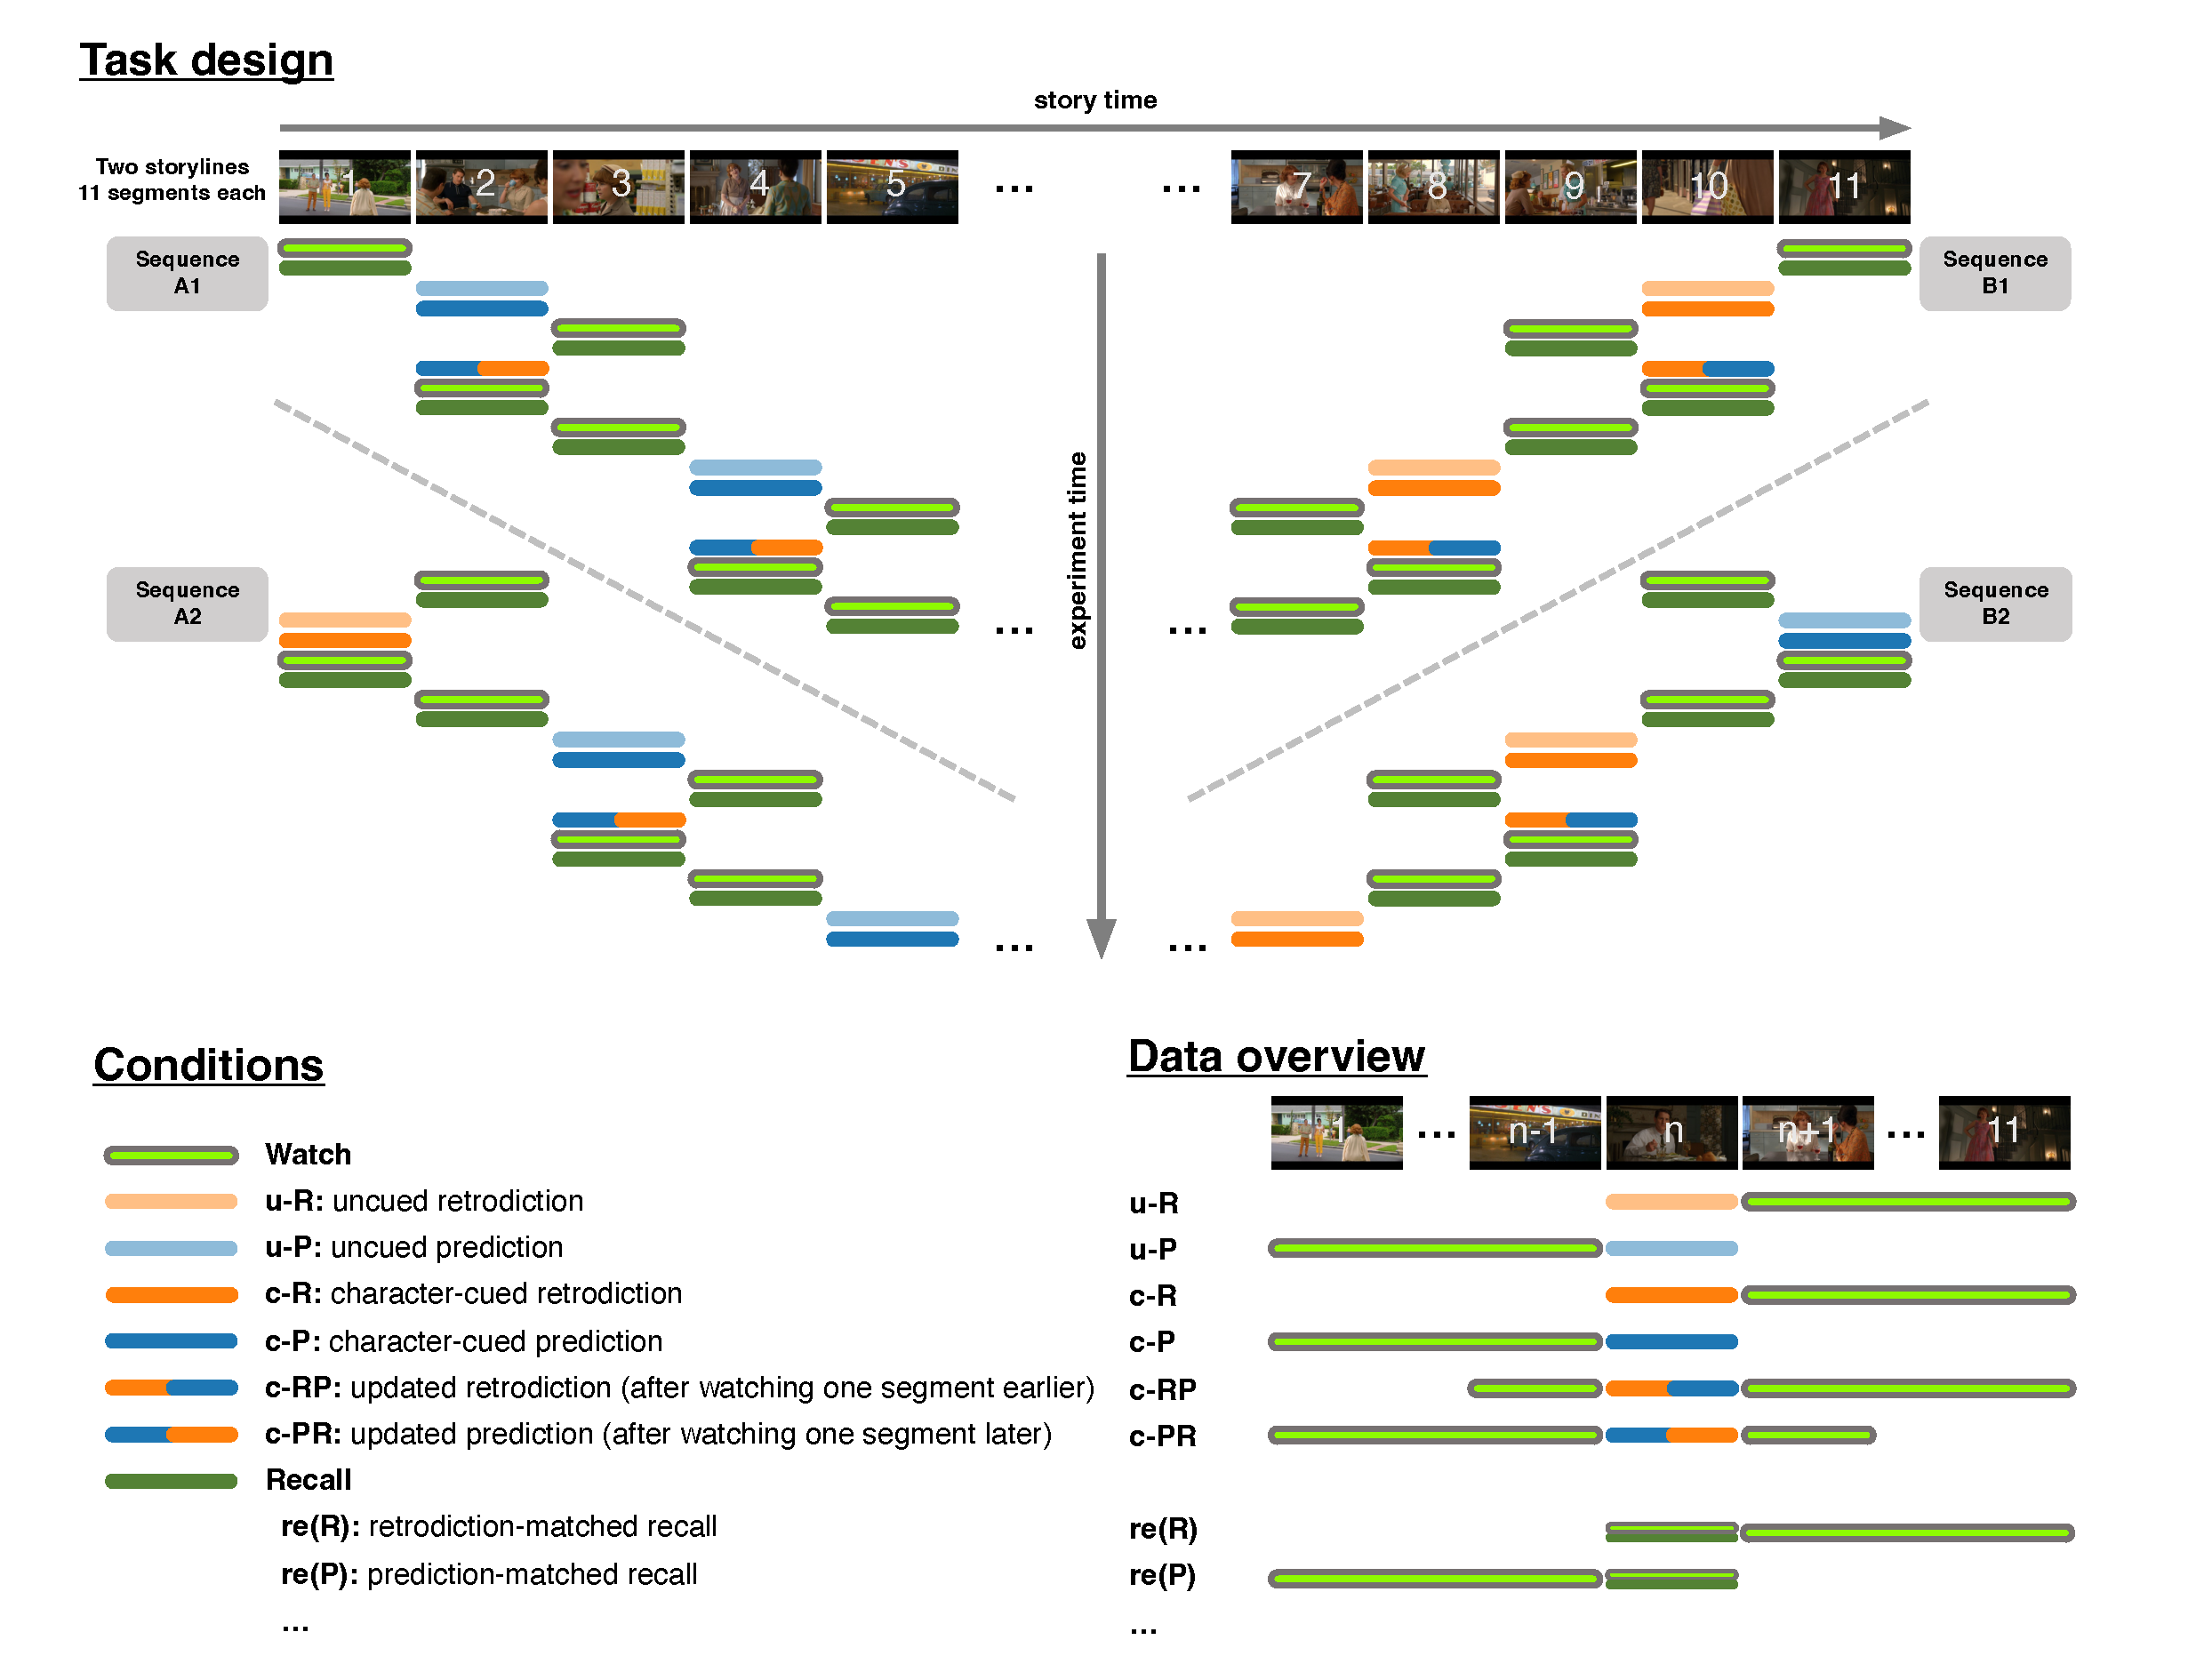
\includegraphics[width=\textwidth]{methods}

  \caption{\textbf{Task overview.} Participants in our main experiment watched
  segments of two storylines from the television series \textit{Why Women
  Kill}. They made free-form text responses to either retrodict what had
  happened in the previous segment, predict what would happen in the next
  segment, or recall what happened in the just-watched segment. Across four
  counterbalanced sequences, we systematically varied whether participants
  watched the segments in forward or reverse chronological order, whether (or
  not) responses were cued using the main characters in the target segment, and
  which other segments participants had watched prior to making a response. For
  each segment, we collected several retrodiction, prediction, and/or recall
  responses across different experimental conditions. Experiment time is
  denoted along the vertical axis, storyline segments are indicated along the
  horizontal axis, and the colors denote experimental tasks (conditions). For
  an analogous depiction of our replication experiment's design, see
  Fig.~\MethodsReplExp.}

  \label{fig:method}
\end{figure}

We asked participants in our main experiment to generate four types of
responses after watching each video segment: uncued responses, character-cued
responses, updated responses, and recalls (Fig.~\ref{fig:method}, \textit{Data
overview}). To generate \textit{uncued} responses, we asked participants to
either retrodict (uncued retrodiction; \textit{u-R}) what happened shortly
before or predict (uncued prediction; \textit{u-P}) what happened shortly after
the just-watched segment. To generate \textit{character-cued} responses, we
asked participants to retrodict (character-cued retrodiction; \textit{c-R}) or
predict (character-cued prediction; \textit{c-P}) what came before or after the
just-watched segment, but we provided additional information to the participant
about which character(s) would be present in the target (to-be-retrodicted or
to-be-predicted) segment. We hypothesized that character-cued responses should
be more accurate than uncued responses, to the extent that participants
incorporate the character information we provided to them into their
retrodictions and predictions. To generate updated responses, we asked
participants to watch an additional segment that came just prior to or just
after the target segment, and then to update their retrodiction (\textit{c-RP})
or prediction (\textit{c-PR}) about the target segment. Results on updated
responses are not reported in this paper. Finally, we also asked participants
to \textit{recall} what happened in the just-watched segment. We labeled these
responses according to which other segments participants had watched prior to
the just-watched target. Retrodiction-matched recall (\textit{re(R)}) responses
were made during the retrodiction sequences (B1 and B2; Fig.~\ref{fig:method}),
whereas prediction-matched recall (\textit{re(P)}) responses were made during
the prediction sequences (A1 and A2; Fig.~\ref{fig:method}). Whereas
retrodiction and prediction responses reflect what participants
\textit{estimate} they would remember after watching the (inferred) target
segment, recall responses provide a benchmark for comparison by measuring what
they \textit{actually} remember about the target segment. Our replication
experiment (Fig.~\MethodsReplExp) used a similar design, but did not have
participants generate recall, re(R), or re(P) responses.

For each retrodiction and prediction, participants were asked to generate at
least one, and not more than three, responses that constituted ``the sorts of
things [the participant would] expect to have remembered if [they] had watched
the [target] segment.'' They were asked to generate multiple responses only if
those additional responses were (in their judgement) of equal likelihood to
occur. On average, participants generated 1.08 responses per prompt; therefore
we chose to consider only participants' first (``most probable'' or ``most
important'') responses to each prompt. We also discarded a small number ($n =
20$) of character-cued responses that did not contain references to all cued
characters, along with one additional response due to the participant's
misunderstanding of the task instructions during that trial. We carried out our
analyses on the remaining 2084 retrodiction, prediction, and recall responses.

\begin{figure}[tp]
  \centering
  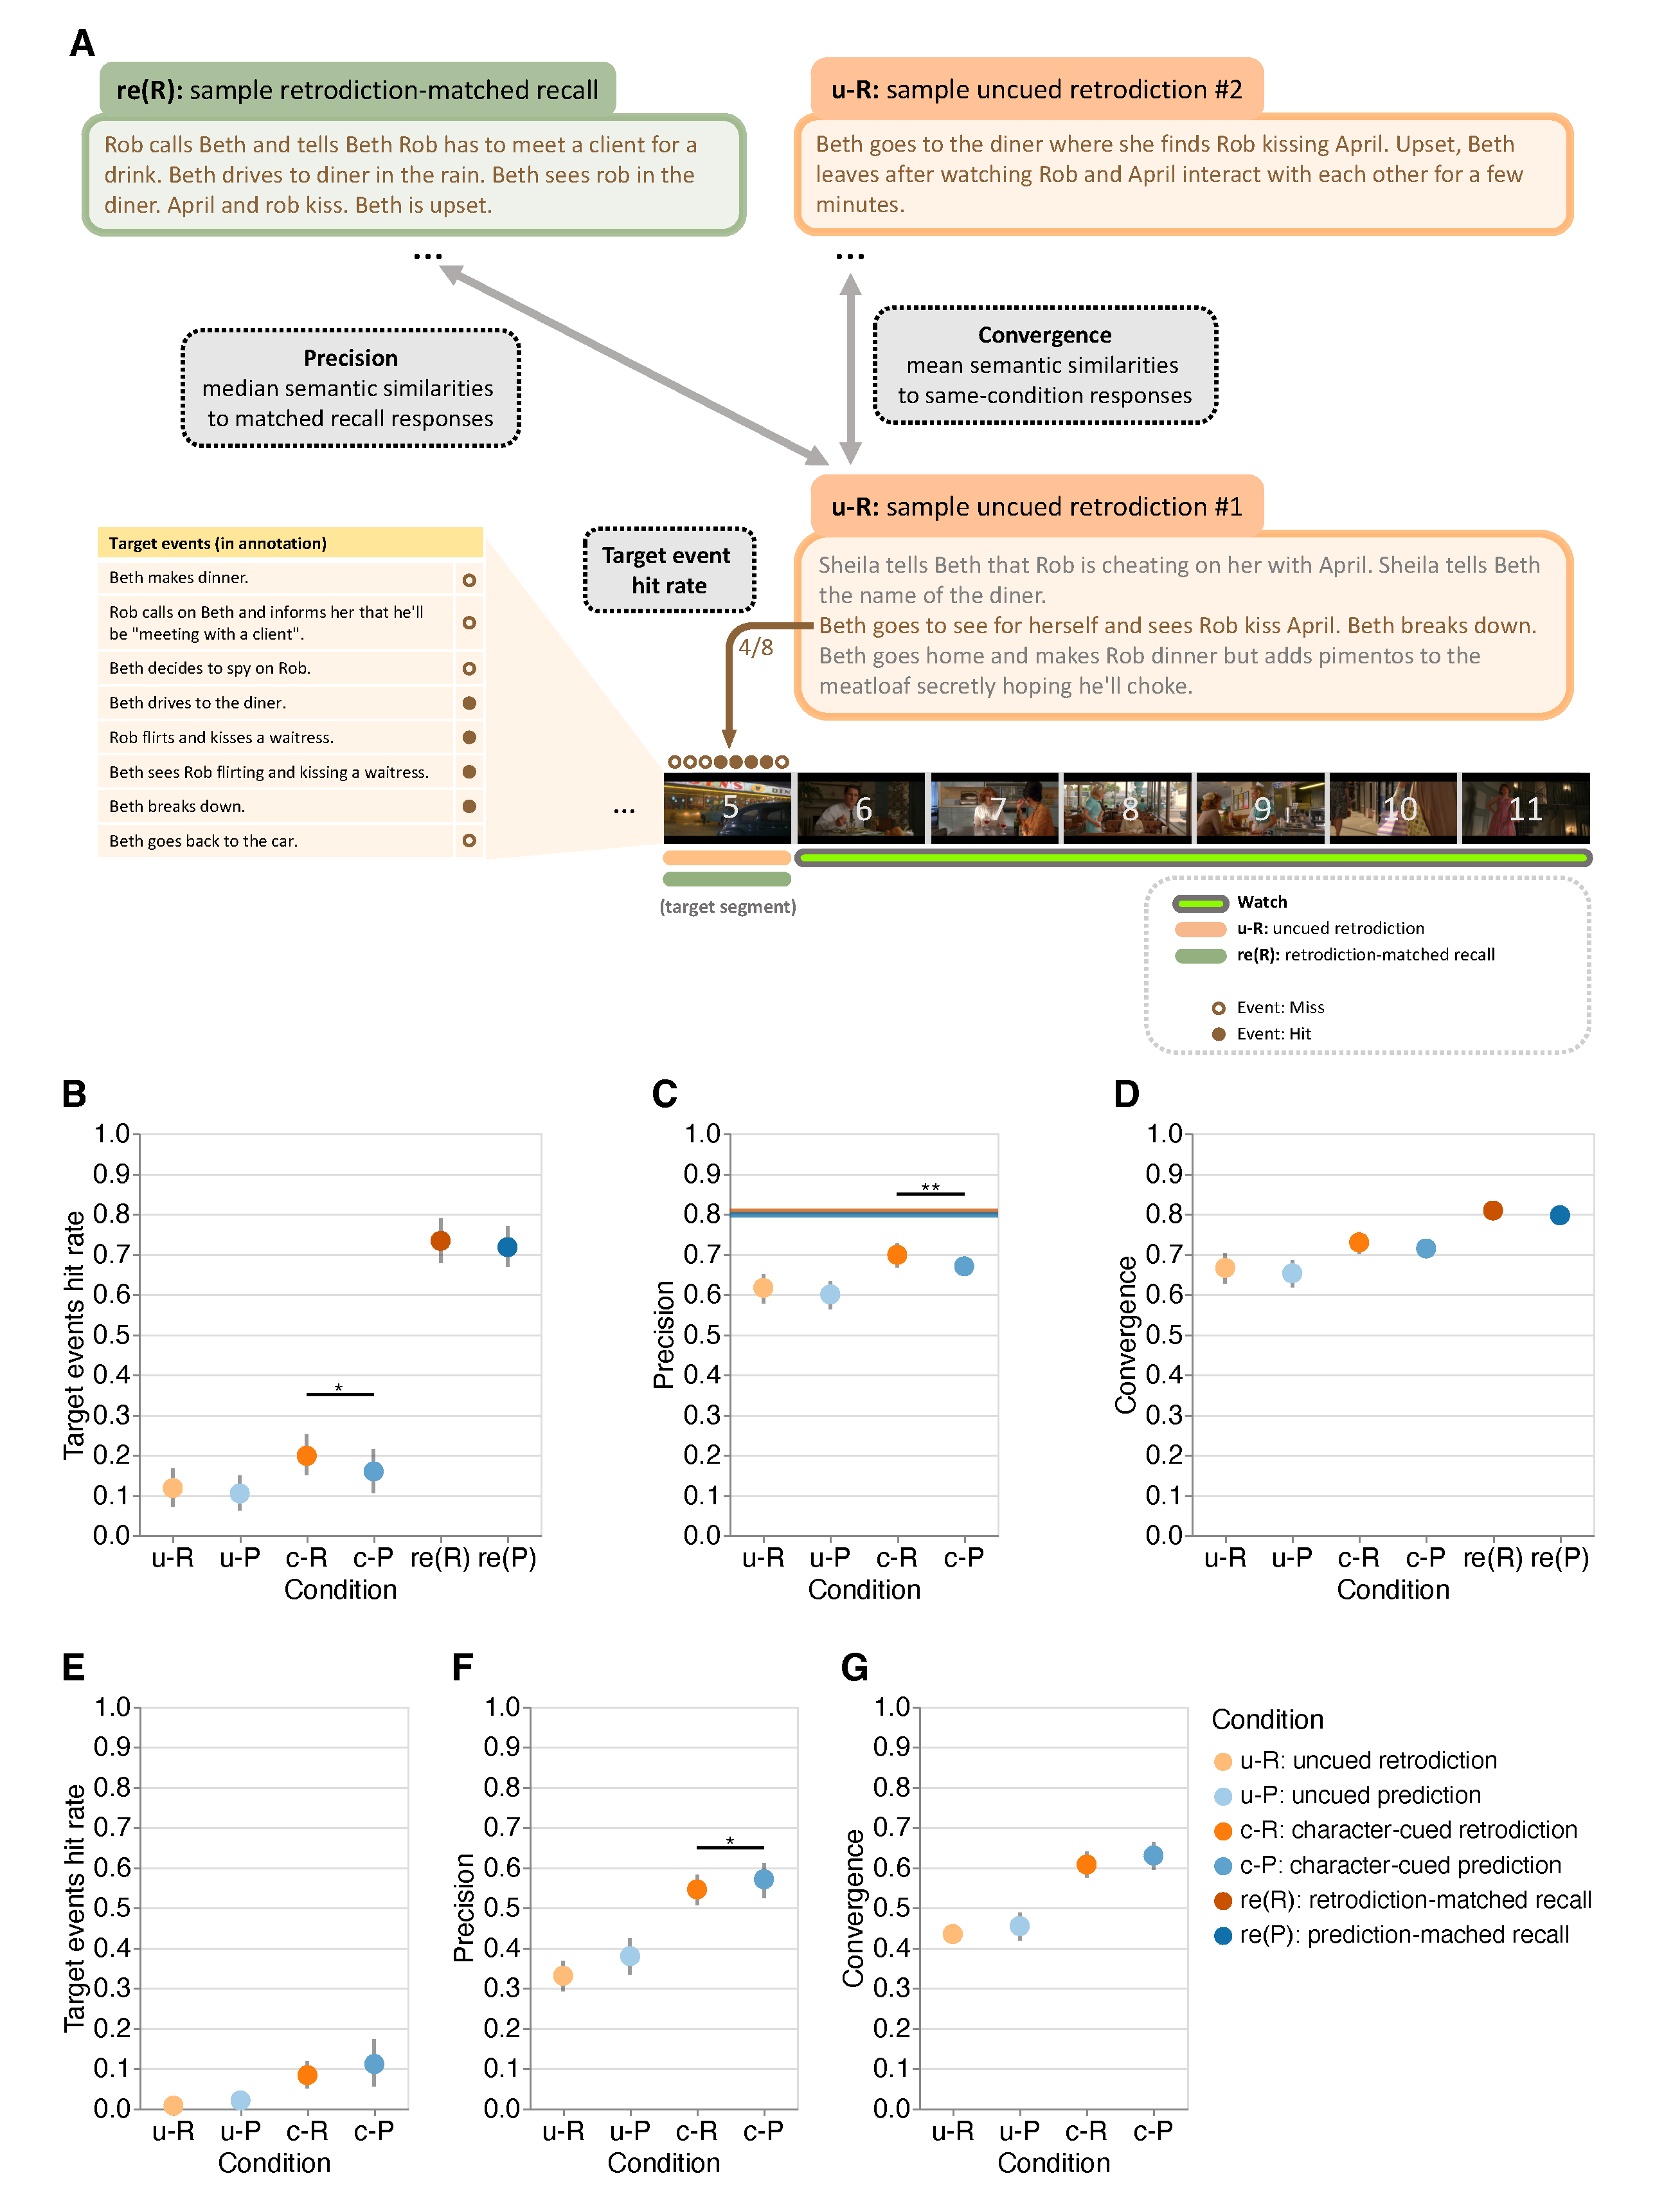
\includegraphics[width=0.80\textwidth]{results1}

  \caption{\textbf{Retrodiction, prediction, and recall performance by
  experimental condition.} \textbf{A. Methods schematic.} For each
  retrodiction, prediction, and recall response, we calculated the hit rate for
  events in the target segment, the response precision (see \textit{Methods}),
  and the response convergence across participants (see \textit{Methods}).
  \textbf{B. Target event hit rate.} Mean proportions of target events that
  were contained in participants' responses, for each response type, averaged
  across target segments. \textbf{C. Response precision.} Mean precisions of
  participants' responses, for each response type, averaged across target
  segments. The horizontal lines denote the mean pairwise semantic similarities
  (see \textit{Methods}) across recall responses (re(R): orange; re(P): blue).
  \textbf{D. Response convergence.} Mean (across-participant) convergence of
  participants' responses, for each response type, averaged across target
  segments. All panels: error bars denote bootstrapped 95\% confidence
  intervals. Asterisks indicate significance in the (generalized) linear mixed
  models: * denotes $p < 0.05$ and ** denotes $p < 0.01$. See
  Figure~\targetAsymmetries for analogous results from our replication
  experiment.}

  \label{fig:result1}
\end{figure}
 
We used two general approaches to assess the quality of participants' responses
(see \textit{Methods}, Figs.~\ref{fig:result1}A). One approach entailed
manually annotating events in the video and counting the number of matched
events in participants' responses. We identified a total of 117 unique events
reflected across the 22 video segments (range: 3--9 per segment; see
\textit{Methods}, Table \stimDescription). We assigned one ``point'' to each of
these video events. We also identified 23 additional events in participants'
responses that were either summaries of several events or that were partial
matches to the manually identified video events. We assigned 0.5 point to each
of these additional events. This point system enabled us to compute the numbers
and proportions (\textit{hit rates}) of correctly retrodicted, predicted, and
recalled events contained in each response. Our second approach entailed using
a natural language processing model~\citep{CerEtal18} to embed annotations and
responses in a 512-dimensional feature space. This approach was designed to
capture conceptual overlap between responses that were not necessarily tied to
specific events. To quantify this conceptual overlap, we computed the
similarities between the embeddings of different sets of responses. Following
\cite{HeusEtal21}, we defined the \textit{precision} of each participants'
retrodictions or predictions about a target segment as the median cosine
similarities between the embeddings of (a) the participant's retrodiction or
prediction response for the target segment and (b) each \textit{other}
participant's recalls of the same segment. In other words, precision is
designed to measure the extent to which retrodictions and predictions captured
the conceptual content that (other) participants remembered. We also developed
a related measure, which we call \textit{convergence}, to characterize response
similarities across participants. In particular, we defined convergence as the
mean cosine similarity between the embeddings of a participant's responses to a
target segment and all other participants' responses (of the same type) to the
same segment. We analyzed the data using generalized linear mixed models, with
participant and stimulus (e.g., target segment) identities as crossed random
effects (see \textit{Methods}).

First we sought to validate a main effect of response type (i.e., uncued
responses, character-cued responses, and recalls), irrespective of the temporal
direction (retrodiction versus prediction). Across these three types of
responses, participants have access to increasing amounts of information about
the target segment. Therefore, across these response types, we hypothesized
that participants' responses should become both more accurate and more
convergent across individuals. Consistent with this hypothesis, participants'
character-cued retrodictions and predictions were associated with higher target
event hit rates than uncued retrodictions and predictions (odds ratio (OR):
2.65, $Z = 4.24$, $p < 0.001$, 95\% confidence interval (CI): 1.69 to 4.16;
Fig.~\ref{fig:result1}B). These character-cued responses were also more precise
($b = 0.13$, $t(18.1) = 9.43$, $p < 0.001$, CI: 0.10 to 0.16;
Fig.~\ref{fig:result1}C) and convergent across individuals ($b = 0.11$,
$t(18.6) = 6.21$, $p < 0.001$, CI: 0.07 to 0.15; Fig.~\ref{fig:result1}D).
Relative to character-cued responses, participants' recalls showed higher
target event hit rates (OR = 21.83, $Z = 10.61$, $p < 0.001$, CI: 12.35 to
38.59) and were more convergence across individuals ($b = 0.20$, $t(19.4) =
9.10$, $p < 0.001$, CI: 0.16 to 0.25). These results are consistent with the
common-sense notion that access to more information about a target segment
yields better performance (i.e., higher hit rates, precision, and convergence
across individuals). These findings also held for our replication experiment
(Fig.~\targetAsymmetries; hit rates of character-cued vs. uncued responses: OR:
XXX, $Z = XXX$, $p = XXX$, 95\% confidence interval (CI): XXX to XXX;
precisions of character-cued vs. uncued responses: $b = XXX$, $t(XXX) = XXX$,
$p = XXX$, CI: XXX to XXX; convergence of character-cued vs. uncued responses:
$b = XXX$, $t(XXX) = XXX$, $p = XXX$, CI: XXX to XXX).

Next we carried out a series of analyses specifically aimed at characterizing
temporal direction effects--- i.e, the relative quality of retrodictions versus
predictions across different types of responses. We hoped that these analyses
might provide insights into our central question about whether inferences about
the past and future are equally accurate. Across both uncued and character-cued
responses in our main experiment (Fig.~\ref{fig:method}), retrodictions had
numerically higher hit rates than predictions (Fig.~\ref{fig:result1}B).
However, these differences were only statistically reliable for character-cued
responses (uncued responses: OR = 1.17, $Z = 0.35$, $p = 0.73$, CI: 0.47 to
2.92; character-cued responses: OR = 1.93, $Z = 2.15$, $p = 0.03$, CI: 1.06 to
3.52). We observed a similar pattern of results for the precisions of
participants' responses (Fig.~\ref{fig:result1}C). Specifically, their
responses tended to be numerically more precise for retrodictions versus
predictions, but the differences were only statistically reliable for
character-cued responses (uncued responses: $b = 0.03$, $t(20.9) = 1.09$, $p =
0.29$, CI: -0.03 to 0.10; character-cued responses: $b = 0.06$, $t(20.8) =
3.01$, $p = 0.007$, CI: 0.02 to 0.11). We also consistently observed
numerically higher convergence across participants for retrodictions versus
predictions (Fig.~\ref{fig:result1}D), but neither of these differences were
statistically reliable (uncued responses: $b = 0.03$, $t(17.9) = 0.75$, $p =
0.46$, CI: -0.05 to 0.11; character-cued responses: $b = 0.04$, $t(17.4) =
1.46$, $p = 0.16$, CI: -0.02 to 0.09). In our replication experiment
(Fig.~\targetAsymmetries), participants were numerically better at making
\textit{predictions} than retrodictions, but none of these differences were
statistically reliable (hit rate for uncued responses: OR = XXX, $Z = XXX$, $p
= XXX$, CI: XXX to XXX; hit rate for character-cued responses: OR = XXX, $Z =
XXX$, $p = XXX$, CI: XXX to XXX; precision for uncued response: $b = XXX$,
$t(XXX) = XXX$, $p = XXX$, CI: XXX to XXX; precision for character-cued
responses: $b = XXX$, $t(XXX) = XXX$, $p = XXX$, CI: XXX to XXX; convergence
for uncued responses: $b = XXX$, $t(XXX) = XXX$, $p = XXX$, CI: XXX to XXX;
convergence for character-cued responses: $b = XXX$, $t(XXX) = XXX$, $p = XXX$,
CI: XXX to XXX). Taken together, our results across our main and replication
experiment suggest that whether participants are better at retrodicting versus
predicting the immediate past or future may be somewhat stimulus specific. We
also verified that this was not solely a consequence of how participants'
memory performance might have been affected by watching different segments (or
making different responses to other segments) across conditions by comparing
recall responses in the retrodiction-matched recall (\textit{re(R)}) and
prediction-matched recall (\textit{re(P)}) conditions. Recall performance in
our main experiment was similar in both conditions (target event hit rate: OR =
1.12, $Z = 1.07$, $p = 0.29$, CI: 0.91 to 1.39; convergence: $b = 0.03$,
$t(19.3) = 1.89$, $p = 0.07$, CI: 0.00 to 0.07). (We did not collect recall
responses in our replication experiment.)

\begin{figure}[tp]
  \centering
  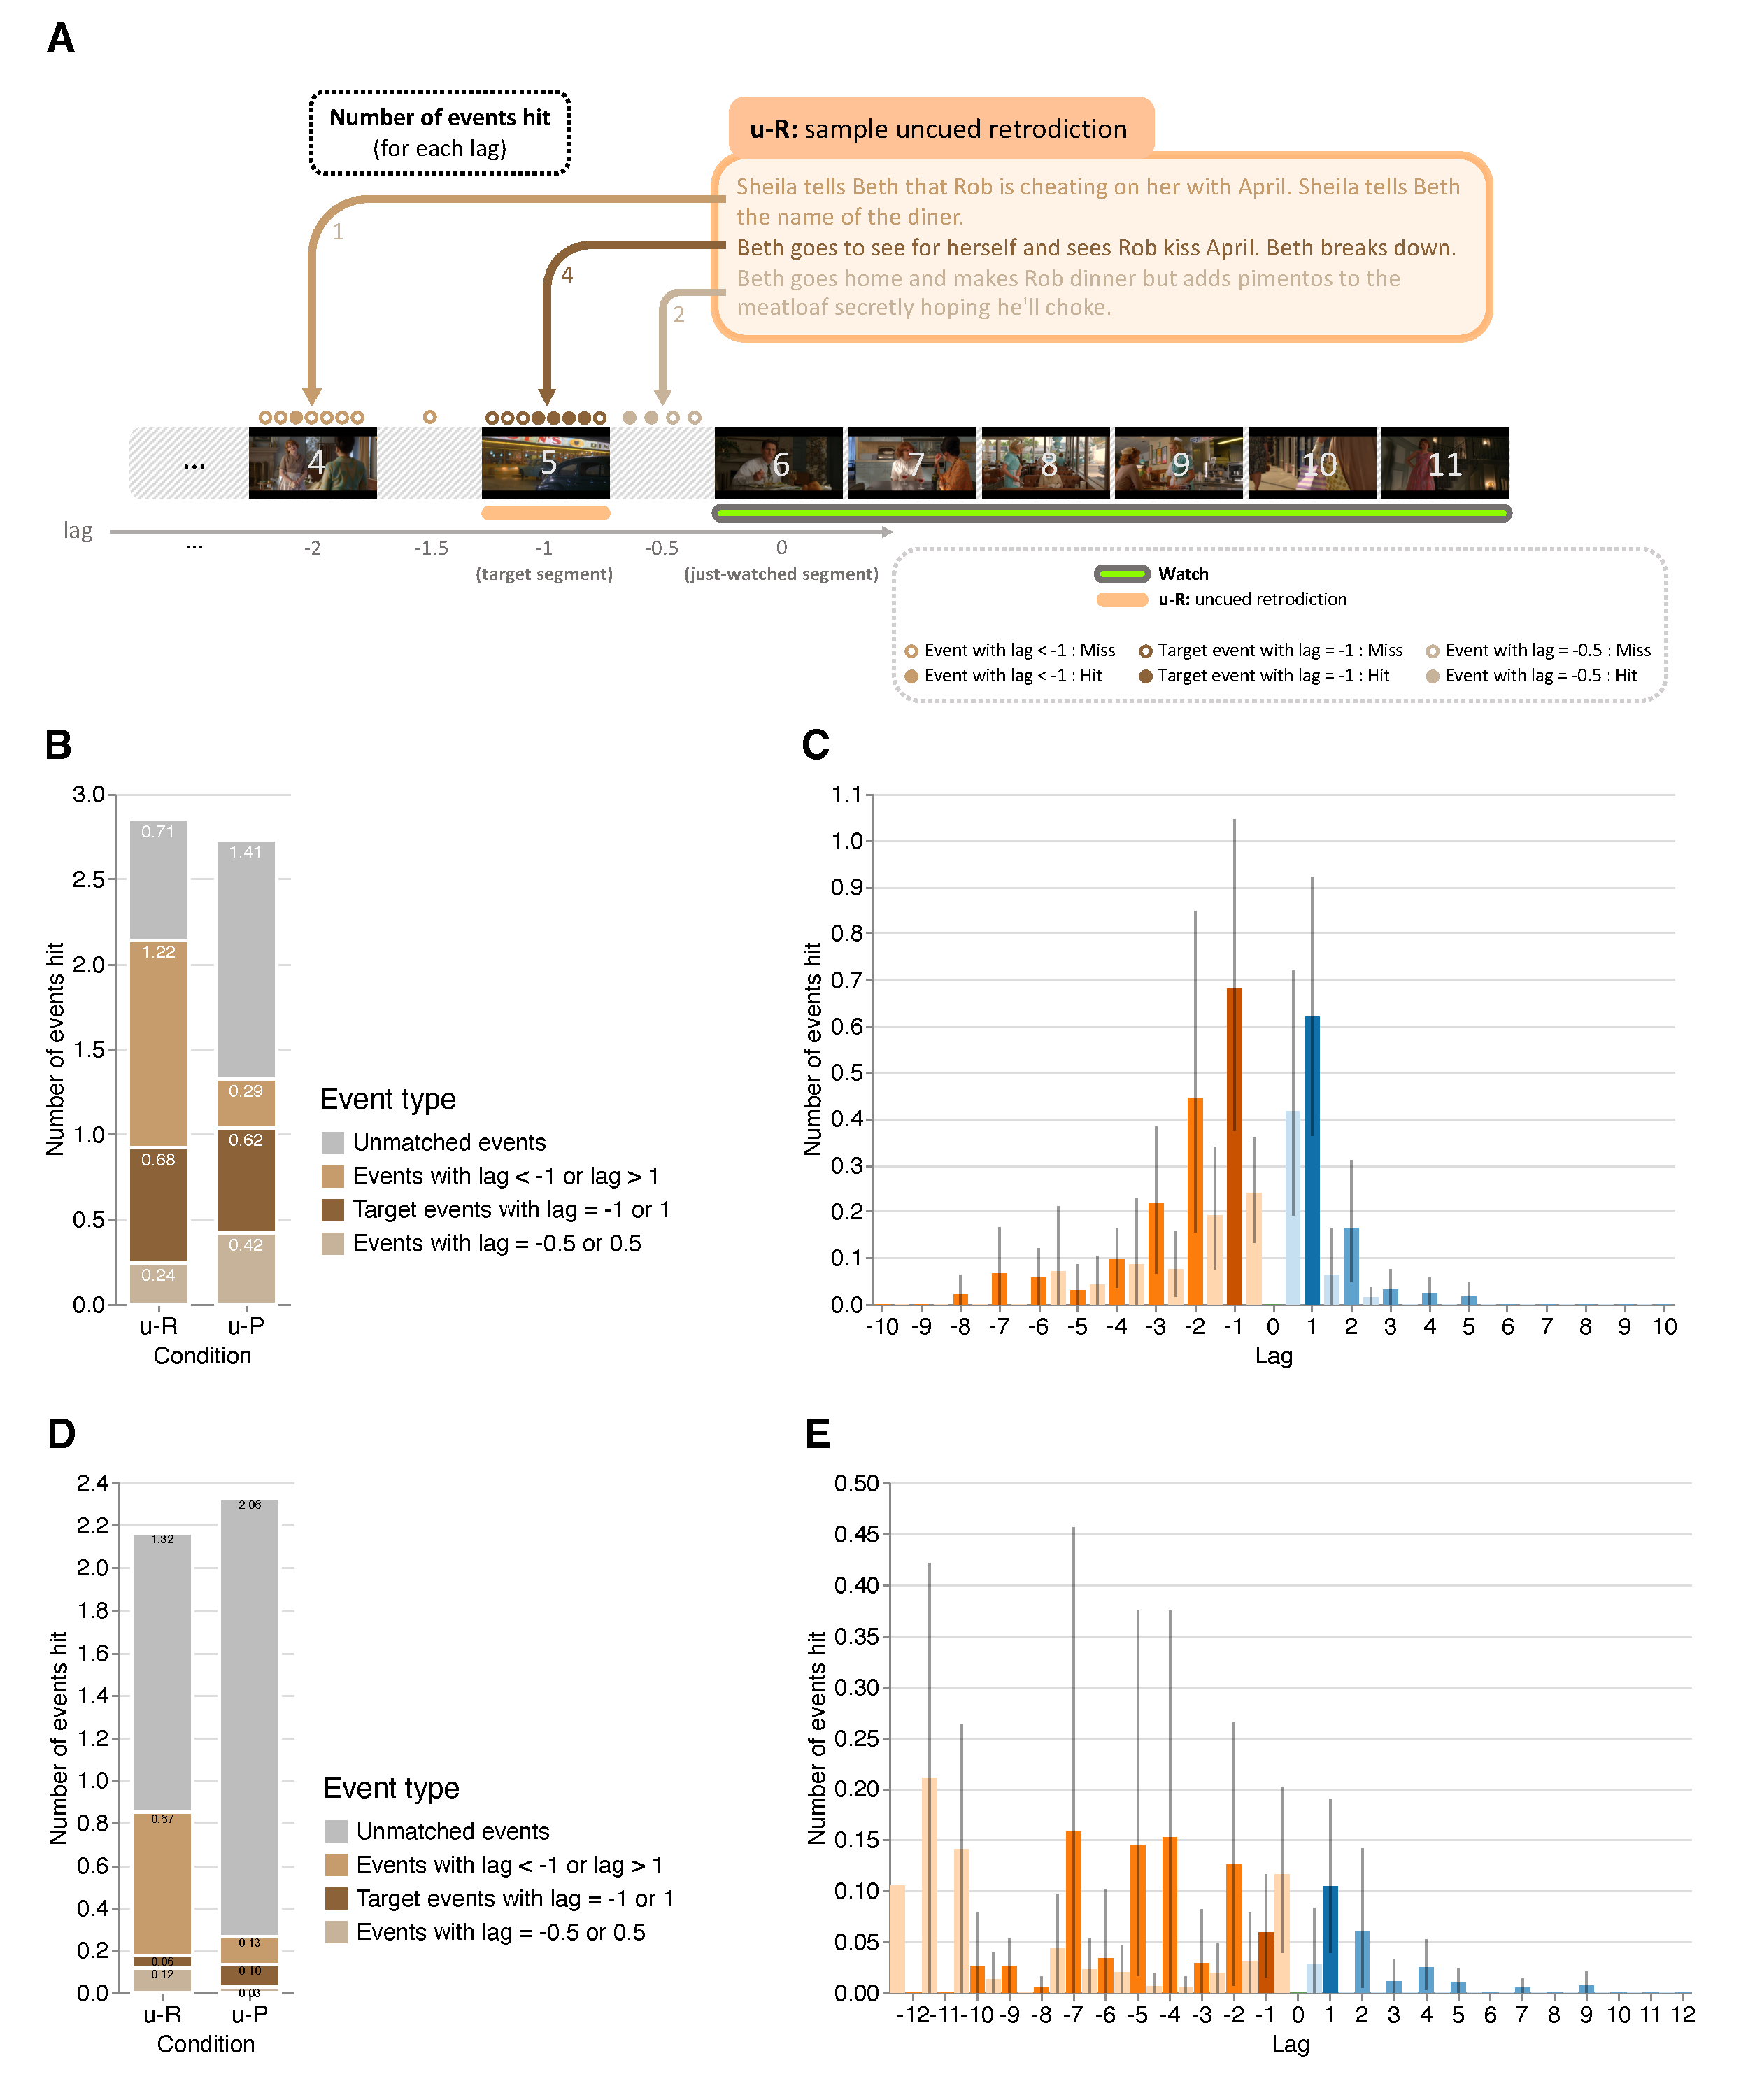
\includegraphics[width=\textwidth]{results2}

  \caption{\textbf{Retrodictions and predictions of temporally near and distant
  events.} \textbf{A. Illustration of annotation approach.} For each uncued
  retrodiction and prediction response in our main experiment, we calculated
  the number of (retrodicted or predicted) events as a function of temporal
  distance from the target segment, or \textit{lag}. Onscreen (explicit) events
  are tagged using integer-valued lags, whereas offscreen (implicit) events are
  tagged using half-step lags ($\pm 0.5$, $\pm 1.5$, etc.). \textbf{B. Number
  of events hit in participants' uncued retrodictions and predictions for each
  event type.} Here we separated events we identified in participants'
  responses according to whether they occurred in the target segment (lags of
  $\pm 1$), during the interval between the target segment and the just-watched
  segment (lags of $\pm 0.5$), at longer temporal distances ($|\mathrm{lag}| >
  1$), or were incorrect (unmatched with any past or future events in the
  narrative). The counts displayed in the panel are averaged across
  just-watched segments. \textbf{C. Number of events hit as a function of
  temporal distance.} Here the (across-segment) mean numbers of events hit in
  participants' uncued retrodictions (orange) and predictions (blue) are
  displayed as a function of temporal distance to the just-watched segment
  (lag). Error bars denote bootstrapped 95\% confidence intervals. Colors
  denote temporal direction (orange: past; blue: future) and distance (darker
  shading: onscreen events from segments adjacent to the target segment;
  lighter shading: offscreen events). See Figure~\hitRates for an analogous
  presentation of results from our replication study.}

  \label{fig:result2}
\end{figure}

The above analyses were focused solely on the target segment (i.e.,
retrodiction of segment $n$ after watching segments $(n+1)... 11$, or
prediction of segment $n$ after watching segments $1 ...(n-1)$). We wondered
whether participants' responses might also contain longer-range information
about preceding or proceeding events. In order to carry out this analysis
properly, we reasoned that participants might reference past or future events
that were \textit{implied} to have occurred offscreen, but not explicitly shown
onscreen. For example, a character in location A during one scene might appear
in location B during the immediately following scene. Although it wasn't shown
onscreen, we can infer that the character traveled between locations A and B
sometime between the time intervals separating the scenes~\citep{Bord08}. In
all, we manually identified a set of 74 \textit{implicit} offscreen events that
were implied to have occurred given what was (explicitly) depicted onscreen
(Fig.~\ref{fig:result2}A), plus one additional partial event and one additional
summary event. We defined the just-watched segment as having a \textit{lag} of
0. We assigned the target segment of a participant's retrodiction or prediction
(i.e., the immediately preceding or proceeding segment) a lag of -1 or +1,
respectively. The segment following the next was assigned a lag of 2, and so
on. We tagged offscreen events using half steps. For example, an offscreen
event that occurred after the prior segment but before the just-watched segment
would be assigned a lag of -0.5.

Because there is no ``ground truth'' number of offscreen events, we could not
compute the hit rates for offscreen events. Instead, we counted up the absolute
\textit{number} of retrodicted or predicted events as a function of lag. In
other words, given that the participant had just watched segment $i$, we asked
how many events from segment $i + lag$ they retrodicted or predicted, on
average, given that they were aiming to retrodict or predict events at lags of
$\pm 1$. We also counted the numbers of \textit{unmatched} events in
participants' responses that did not correspond to any events in the relevant
segments of the narrative. We focused specifically on \textit{uncued}
retrodictions and predictions, which we hypothesized would provide the cleanest
characterizations of participants' initial estimates of the unobserved past and
future (i.e., without potential biases introduced by additional character
information, as in the character-cued responses). For participants in our main
experiment, the numbers of uncued retrodicted and predicted target (lag = $\pm
1$) events were not reliably different (OR = 0.92, $Z = -0.15$, $p = 0.88$, CI:
0.30 to 2.84). In other words, uncued retrodictions and predictions over short
timescales did not exhibit reliable asymmetries. This ``null result'' also held
in our replication study (OR = XXX, $Z = XXX$, $p = XXX$, CI: XXX to XXX).
However, when retrodicting, participants in both experiments mentioned events
from the distant past ($\mathrm{lag} < -1$) more often than participants
predicted events from the distant future ($\mathrm{lag} > 1$; main experiment:
OR = 9.10, $Z = 3.80$, $p < 0.001$, CI: 2.92 to 28.39; Fig.~\ref{fig:result2}B,
C; replication experiment: OR = XXX, $Z = XXX$, $p = XXX$, CI: XXX to XXX;
Fig.~\hitRates; for results from the character-cued conditions, see
Fig.~\events). Despite this asymmetry in the accuracies of participants'
long-range retrodictions versus predictions, there were no reliable differences
in the \textit{numbers} of uncued retrodicted versus predicted events (across
all lags; main experiment: OR = 1.05, $Z = 0.75$, $p = 0.45$, CI: 0.93 to 1.18;
replication experiment: OR = XXX, $Z = XXX$, $p = XXX$). Nor did we find any
reliable differences in the numbers of offscreen events immediately before or
after the just-watched segment ($lag = \pm 0.5$; main experiment: OR = 0.75, $Z
= -0.36$, $p = 0.72$, CI: 0.15 to 3.59; replication experiment: OR = XXX, $Z =
XXX$, $p = XXX$, CI: XXX to XXX). The apparent discrepancy between
participants' asymmetric accuracy but symmetric event counts was due to
participants' tendencies to reference ``unmatched'' events (i.e., events that
did not correspond to any explicit or implicit event in the story) more in
their predictions than retrodictions (main experiment: OR = 0.36, $Z = -4.53$,
$p < 0.001$, CI: 0.23 to 0.56; replication experiment: OR = XXX, $Z = XXX$, $p
= XXX$, CI: XXX to XXX). We confirmed that the retrodiction advantage held when
controlling for absolute lag (main experiment: OR = 34.31, $Z = 3.28$, $p =
0.001$, CI: 4.16 to 283.20; replication experiment: OR = XXX, $Z = XXX$, $p =
XXX$, CI: XXX to XXX), for onscreen events alone (main experiment: OR = 47.54,
$Z = 3.74$, $p < 0.001$, CI: 6.27 to 360.60; replication experiment: OR = XXX,
$Z = XXX$, $p = XXX$, CI: XXX to XXX), and marginally for offscreen events
alone (main experiment: OR = 24.76, $Z = 1.71$, $p = 0.09$, CI: 0.63 to 975.27;
replication experiment: OR = XXX, $Z = XXX$, $p = XXX$, CI: XXX to XXX). Taken
together, these analyses show that (in generating uncued responses)
participants tend to reach ``further'' into the unobserved past, and with
greater accuracy, than the unobserved future.

What might be driving participants to retrodict further and more accurately
into the unobserved past, compared with their predictions of the unobserved
future? By inspecting the video content, we noticed that characters in the
television show frequently referenced both past events and (planned or
predicted) future events in their spoken conversations. We wondered whether the
characters' references might show temporal asymmetries that might explain
participants' behaviors. Across all of the characters' conversations, and
across all of the video segments, we manually identified a total of 82
references to past or future events (i.e., that occurred onscreen or offscreen
before or after the events depicted in the current segment;
Figs.~\ref{fig:result3}A, \references A, \characterRefs). Characters in our
main experiment's stimulus tended to reference the past (52 references) more
than the future (30 references), consistent with previous
work~\citep{DemiEtal18}. References to the past were also skewed to more
temporally distant events compared with references to the future
(Figs.~\ref{fig:result3}B,~\references B,~\characterRefs). These asymmetries
also held for characters in the replication experiment's stimulus
(Fig.~\ref{fig:meta-analysis}). These observations indicate that the characters
in the stimulus display a preference for the past (versus future) in their
conversations. Might this asymmetry be driving the asymmetries in participants'
retrodictions versus predictions?

\begin{figure}[tp]
  \centering
  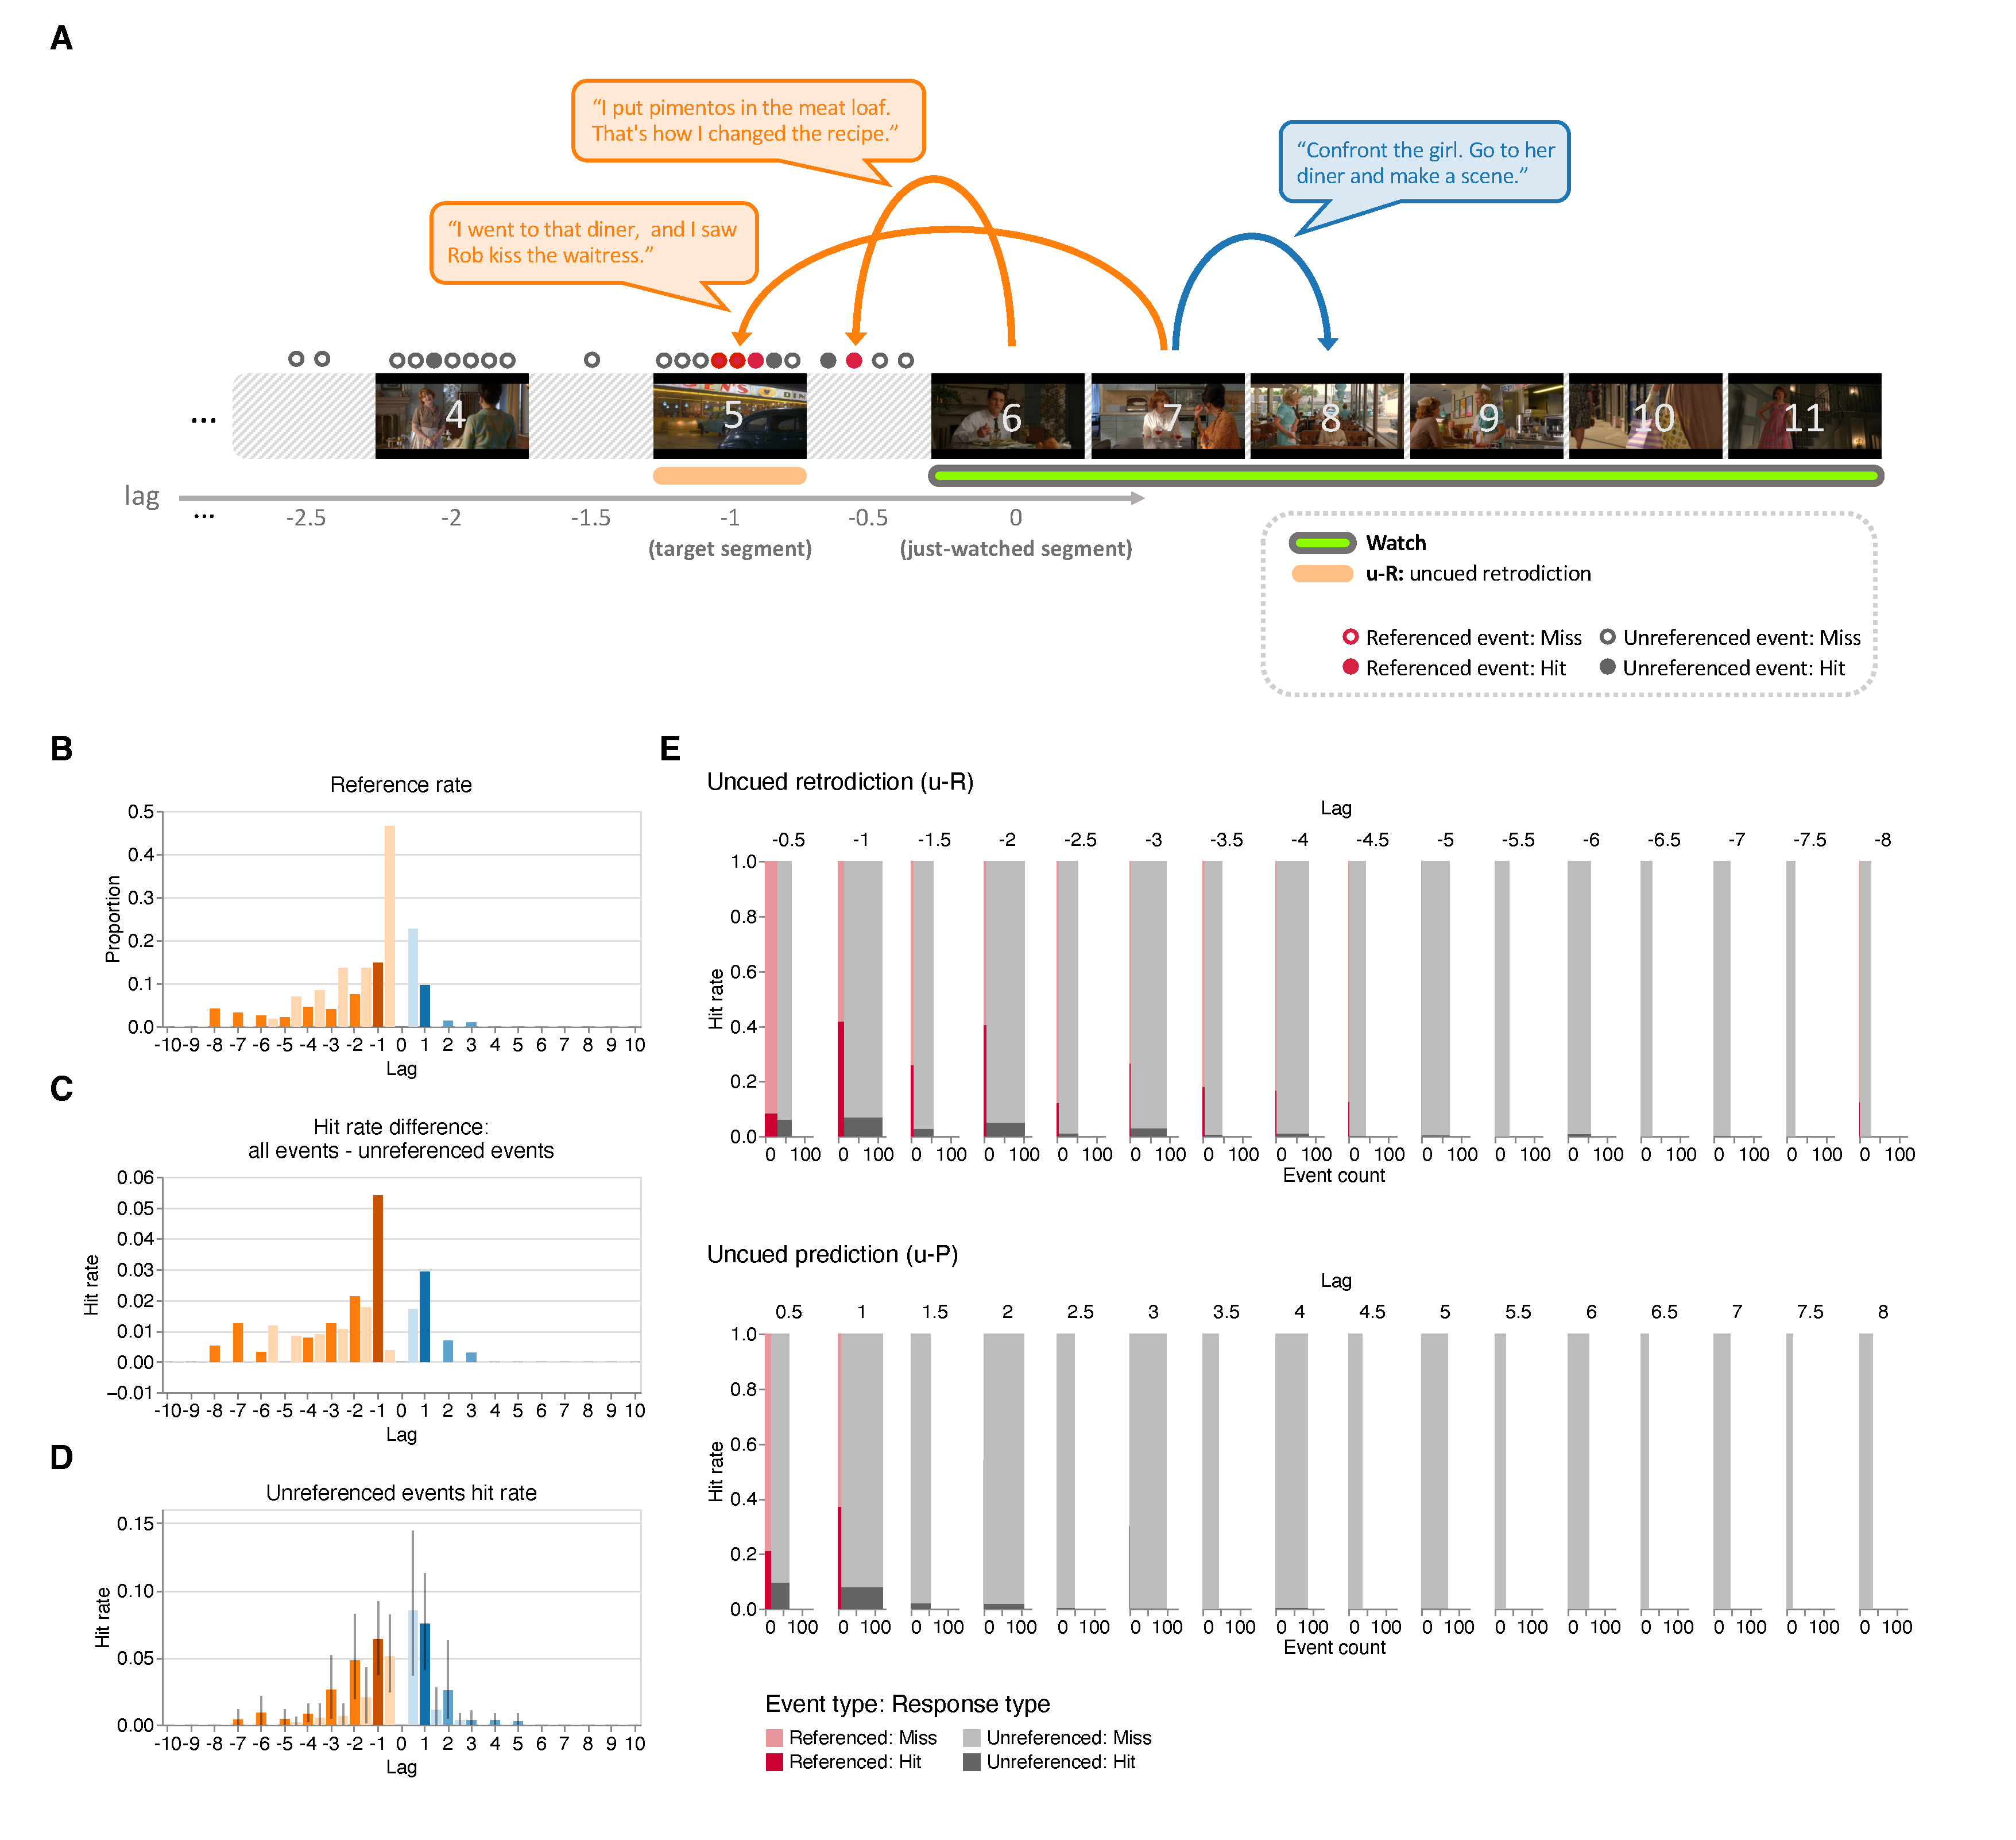
\includegraphics[width=0.9\textwidth]{results3}

  \caption{\textbf{Characters' references drive participants' retrodiction and
  prediction performance.} \textbf{A. Illustration of annotation approach.} We
  manually annotated references to events in past or future segments in
  characters' spoken conversations. We matched each such reference with its
  corresponding storyline event (and its corresponding segment number for
  onscreen events, or half-step segment number for offscreen events). We then
  tracked the hit rate separately for referenced versus unreferenced events in
  participants' uncued retrodictions and predictions. \textbf{B. Reference rate
  as a function of lag.} Across all possible just-watched segments (lag 0), the
  bar heights denote the average proportions of events referenced in other past
  (orange, negative lags) or future (blue, positive lags) segments in our main
  experiment's stimulus. \textbf{C. Difference in hit rates between all events
  and unreferenced events.} To highlight the effect of characters' references
  to past and future events on participants' retrodictions and predictions,
  here we display the difference in across-segment mean hit rates between all
  events and unreferenced events, as a function of temporal distance (lag) to
  the just-watched segment. \textbf{D. Hit rates for unreferenced events.} The
  average response hit rates for unreferenced events are displayed as a
  function of temporal distance to the just-watched segment. Error bars denote
  bootstrapped 95\% confidence intervals. Panels B--D: colors are described in
  the Figure~\ref{fig:result2} caption. \textbf{E. Hit rates and counts of
  referenced and unreferenced events.} As a function of temporal distance to
  the just-watched segment, the sub-panels display the across-segment mean
  numbers ($x$-axes) and hit rates ($y$-axes) of referenced (red) and
  unreferenced (gray) events that participants hit (darker shading) or missed
  (lighter shading) in their uncued retrodictions (top sub-panel) and uncued
  predictions (bottom sub-panel). For an analogous presentation of results from
  the replication experiment, see Fig.~\characterRefs.}

  \label{fig:result3}
\end{figure}

Controlling for temporal distance (lag), past and future events that story
characters referenced in their conversations were associated with higher hit
rates than unreferenced events in our main experiment (uncued retrodiction: OR
= 12.70, $Z = 10.94$, $p < 0.001$, CI: 8.06 to 20.03; uncued prediction: OR =
8.29, $Z = 6.83$, $p < 0.001$, CI: 4.52 to 15.20; Fig.~\ref{fig:result3}E).
This indicates that participants' responses are at least partially influenced
by the characters' conversations. To estimate the contributions of characters’
references on hit rates, we computed the difference in hit rates between all
events (which comprised both referenced and unreferenced events) and
unreferenced events, as a function of lag. These differences exhibited a
temporal asymmetry in favor of retrodiction (Figs.~\ref{fig:result3}C). This
indicates that the asymmetries in participants' retrodictions versus
predictions are also at least partially influenced by the characters'
conversations. However, these temporal asymmetries in participants'
retrodictions and predictions persisted even for events that characters never
referenced in their conversations (hit rates of uncued retrodicted versus
predicted unreferenced events: OR = 2.00, $Z = 2.40$, $p = 0.02$, CI: 1.14 to
3.51; Fig.~\ref{fig:result3}D). When we further separated the unreferenced
events into onscreen events and offscreen events, we found that these
asymmetries held only for the onscreen events (onscreen: OR = 2.65, $Z = 2.59$,
$p = 0.01$, CI: 1.27 to 5.54; offscreen: OR = 1.50, $Z = 0.91$, $p = 0.36$, CI:
0.63 to 3.62). We found similar patterns in our replication experiment
(Fig.~\characterRefs; hit rates of uncued retrodictions for referenced events:
OR = XXX, $Z = XXX$, $p = XXX$, CI: XXX to XXX; uncued predictions for
referenced events: OR = XXX, $Z = XXX$, $p = XXX$, CI: XXX to XXX; hit rates of
uncued retrodcitions for \textit{unreferenced} events: OR = XXX, $Z = XXX$, $p
= XXX$, CI: XXX to XXX; for predicted events: OR = XXX, $Z = XXX$, $p = XXX$,
CI: XXX to XXX). Taken together, these analyses suggest that asymmetries in the
number of references characters make to past and future events partially (but
not entirely) explain why participants tend to retrodict the past further and
more accurately than they predict the future.

\begin{figure}[tp]
  \centering
  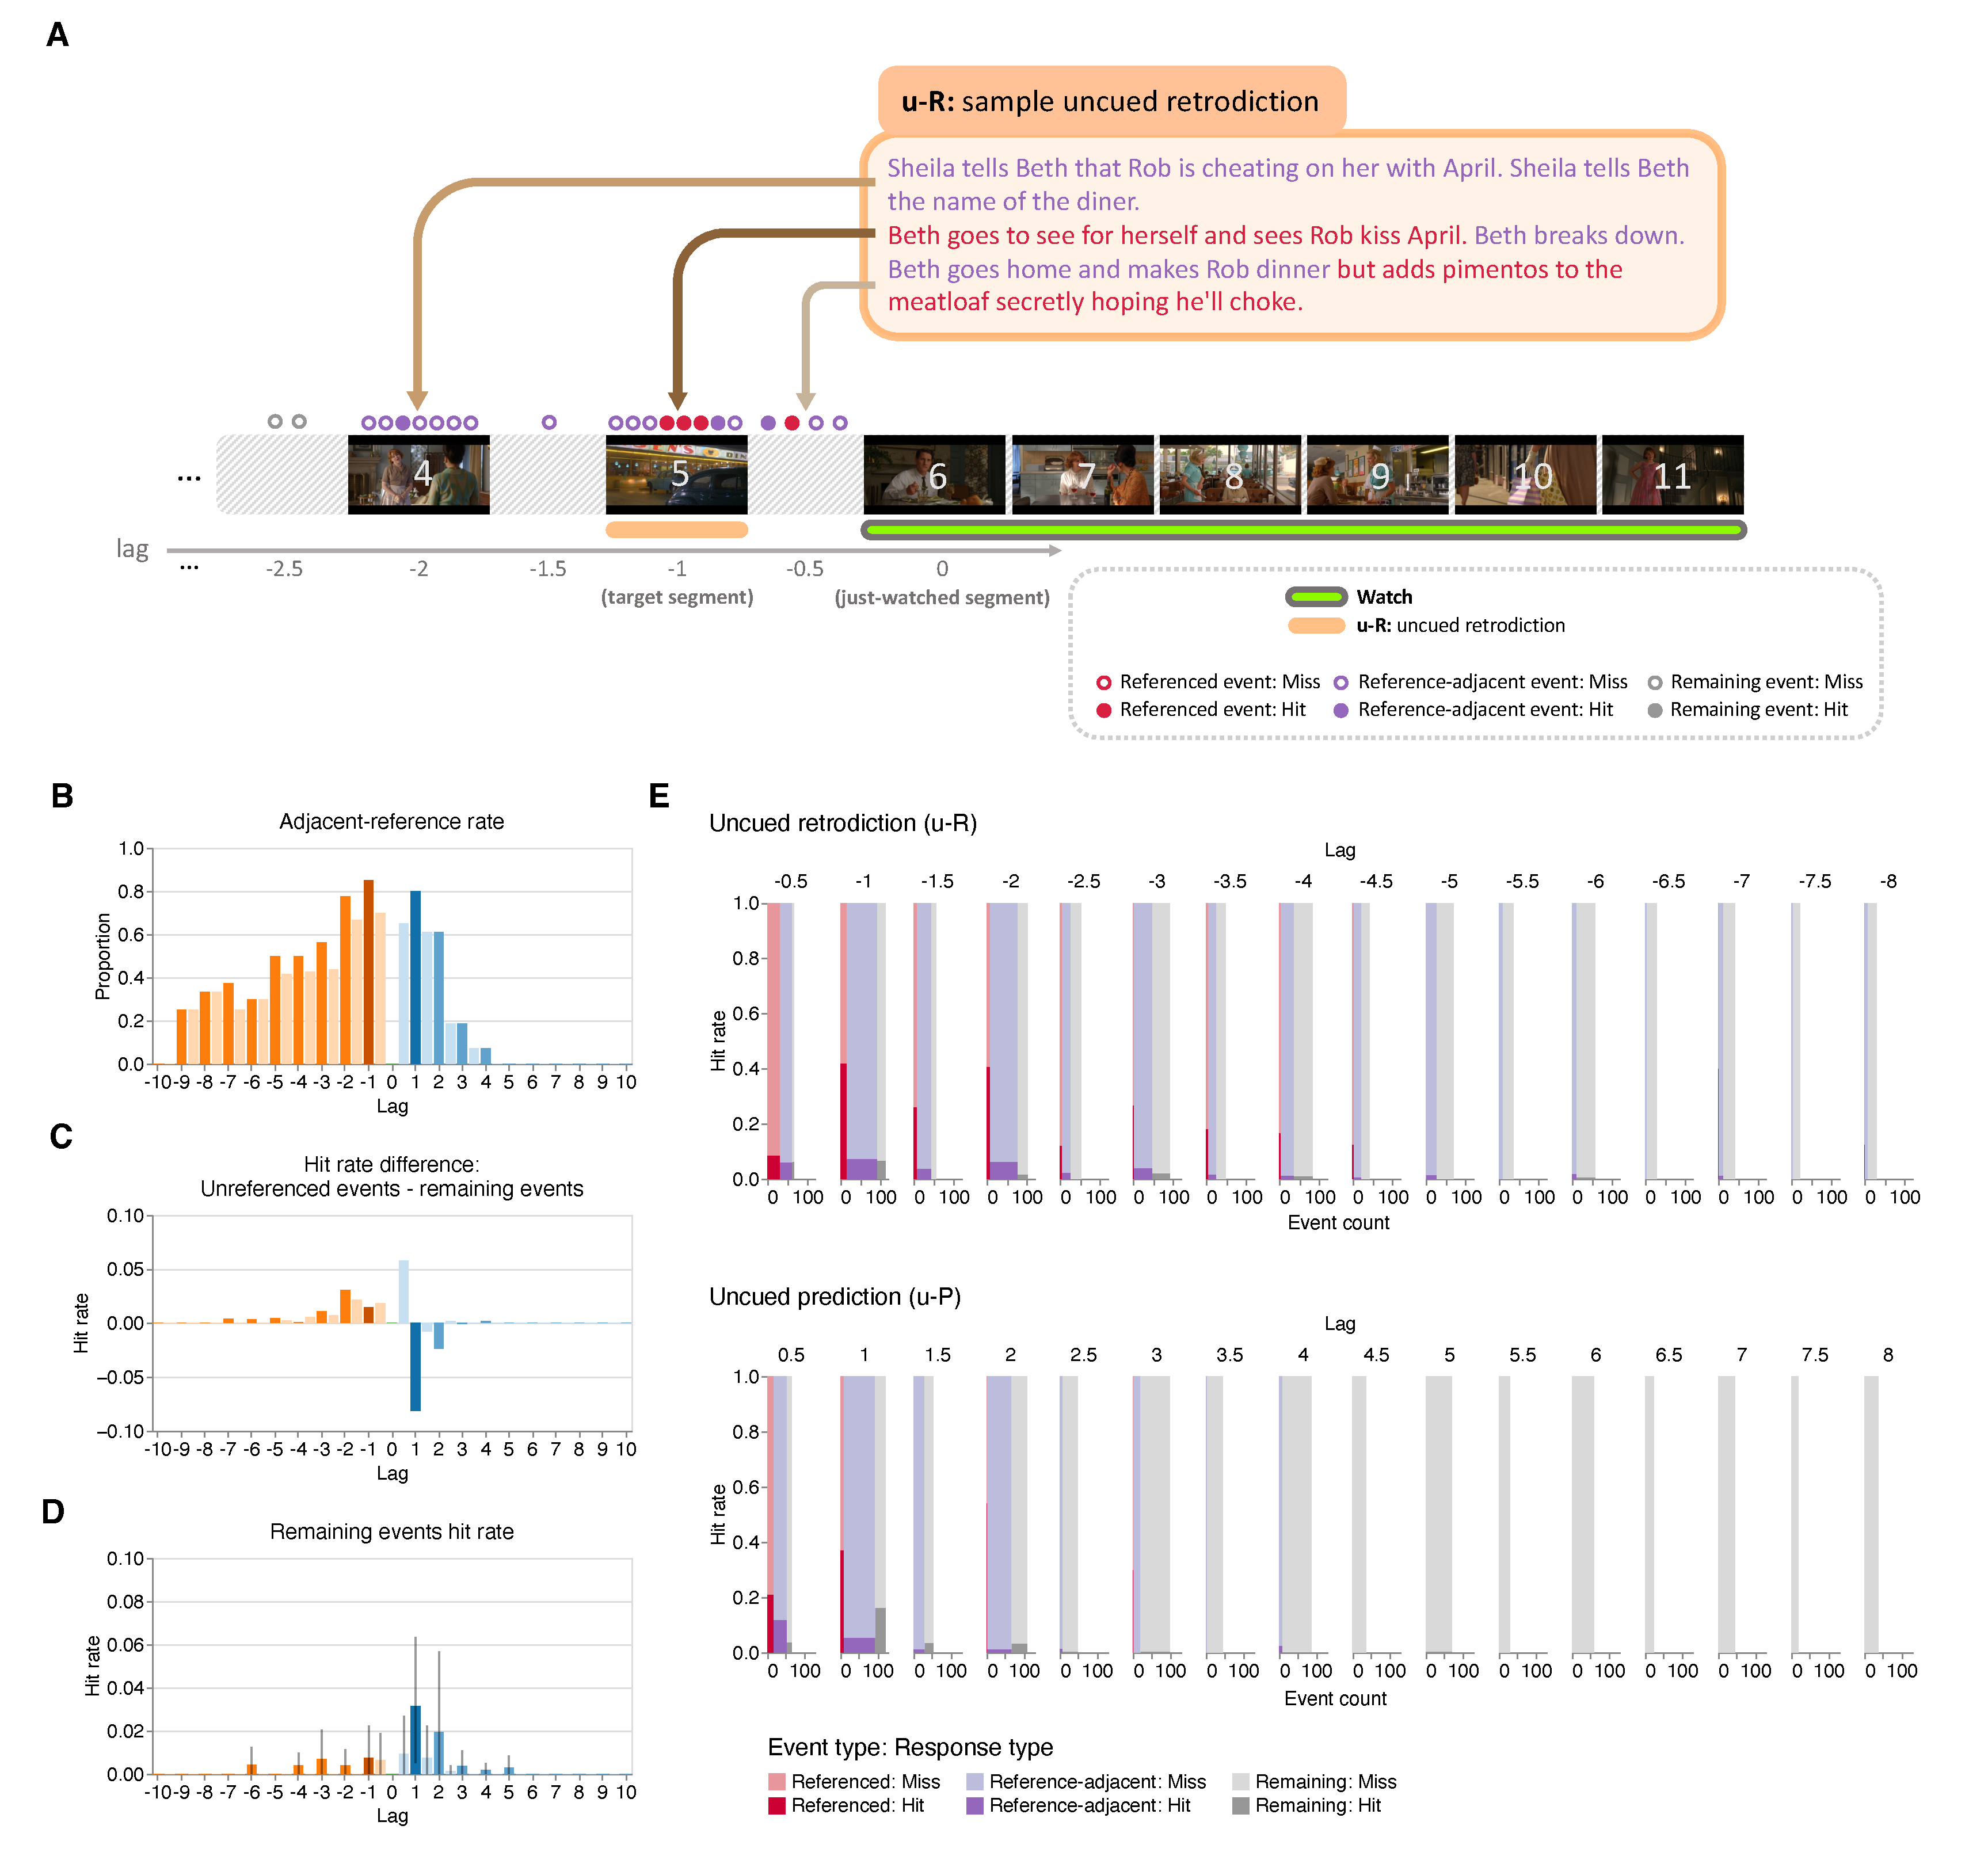
\includegraphics[width=0.8\textwidth]{results4}

  \caption{\textbf{Reference-adjacent events are associated with higher hit
  rates (main experiment).} \textbf{A. Illustration of annotation approach.} We
  extended the annotation procedure depicted in Figure~\ref{fig:result3}A to
  also label unreferenced events that were either temporally adjacent to (i.e.,
  immediately preceding or proceeding) a referenced event (reference-adjacent
  events) or not (remaining events). \textbf{B. Adjacent reference rate for
  unreferenced events as a function of lag.} Across all possible just-watched
  segments (lag 0), the bar heights denote the average proportion of
  unreferenced events in other past (orange, negative lags) or future (blue,
  positive lags) segments that were temporally adjacent to any referenced
  event. \textbf{C. Difference in hit rates between unreferenced events and
  remaining events.} To highlight the effect of reference adjacency on
  retrodiction and prediction of unreferenced events, here we display the
  difference in across-segment mean hit rates between unreferenced events and
  remaining events, as a function of temporal distance (lag) to the
  just-watched segment. \textbf{D. Hit rates for remaining events.} The
  across-segment mean response hit rates for unreferenced events that were
  \textit{not} temporally adjacent to any referenced events are displayed as a
  function of temporal distance to the just-watched segment. Error bars denote
  bootstrapped 95\% confidence intervals. Panels B--D: colors are described in
  the Figure~\ref{fig:result2} caption. \textbf{E. Hit rates and counts of
  referenced, reference-adjacent, and remaining events.} As a function of
  temporal distance to the just-watched segment, the sub-panels display the
  numbers ($x$-axes) and proportions ($y$-axes) of referenced (red),
  reference-adjacent (purple), and remaining (gray) events that participants
  hit (darker shading) or missed (lighter shading) in their uncued
  retrodictions (top sub-panel) and uncued predictions (bottom sub-panel). For
  an analogous depiction of results from our replication experiment see
  Fig.~\refAdjacent.}

  \label{fig:result4}
\end{figure}

If characters' direct references cannot fully account for the temporal
asymmetry in retrodicting the unobserved past versus predicting the unobserved
future, what other factors might explain this phenomenon? The results above
indicate that characters’ references to specific unobserved events in the past
or future boost participants’ estimates of these events. But might characters'
references have other effects on participants' responses \textit{beyond} the
referenced events? For example, real-world experiences and events in realistic
narratives are often characterized by temporal autocorrelations (i.e., what is
``happening now'' will likely relate to what happens ``a moment from now,'' and
so on). Real-world experiences and realistic narratives are also often
structured into ``schemas'' whereby experiences unfold according to a
predictable pattern or formula that characterizes a particular situation, such
as going to a restaurant or catching a flight at the
airport~\citep{BaldEtal18}. If there are associations or temporal dependencies
between temporally nearby events in the television show participants watched,
participants might be able to pick up on these patterns in forming their
responses. This would be reflected in an inference ``boost'' for events that
were \textit{nearby in time} to events that characters referred to in their
conversations, in addition to the referenced events themselves
(Fig.~\ref{fig:result4}A).

Because characters tended to refer to past events more often than future
events, the proportions of unreferenced events that were adjacent to referenced
events should show a similar temporal asymmetry in favor of the past. We tested
this intuition by computing the proportions of unreferenced events in the
stimulus that were temporally adjacent to past or future events referenced by
the characters during a given segment. Here we defined \textit{temporally
adjacent} as any event within an absolute lag of one relative to a referenced
onscreen event, or within an absolute lag of 0.5 to a referenced offscreen
event. We also defined \textit{remaining} events as unreferenced events that
were not temporally adjacent to any referenced events. As shown in
Figure~\ref{fig:result4}B, in our main experiment we observed higher
proportions of unreferenced past than future events that were temporally
adjacent to referenced events. Further, these reference-adjacent events had
higher hit rates than remaining events after controlling for absolute lag
(uncued retrodiction: OR = 7.15, $Z = 2.40$, $p = 0.02$, CI: 1.44 to 35.58;
uncued prediction: OR = 3.11, $Z = 2.30$, $p = 0.02$, CI: 1.18 to 8.21;
Fig.~\ref{fig:result4}E). These findings also held in our replication
experiment (uncued retrodiction: OR = XXX, $Z = XXX$, $p = XXX$, CI: XXX to
XXX; uncued prediction: OR = XXX, $Z = XXX$, $p = XXX$, CI: XXX to XXX;
Fig.~\refAdjacent). To estimate the contributions of reference adjacency on hit
rates, we computed the difference in hit rates between unreferenced events
(which comprised both reference-adjacent and remaining events) and remaining
events, as a function of lag. These differences exhibited a temporal asymmetry
in favor of retrodiction. This suggests that reference-adjacent events also
contribute to participants' retrodiction advantage. Remaining events did
\textit{not} exhibit a reliable temporal asymmetry (main experiment: OR = 0.75,
$Z = 0.33$, $p = 0.74$, CI: 0.14 to 4.08, Fig.~\ref{fig:result4}D; replication
experiment: OR = XXX, $Z = XXX$, $p = XXX$, CI: XXX to XXX, Fig.~\refAdjacent
D), suggesting that, after accounting for temporal adjacency, character's
references to past and future events can explain participants' retrodiction
advantage.

\begin{figure}[tp]
  \centering
  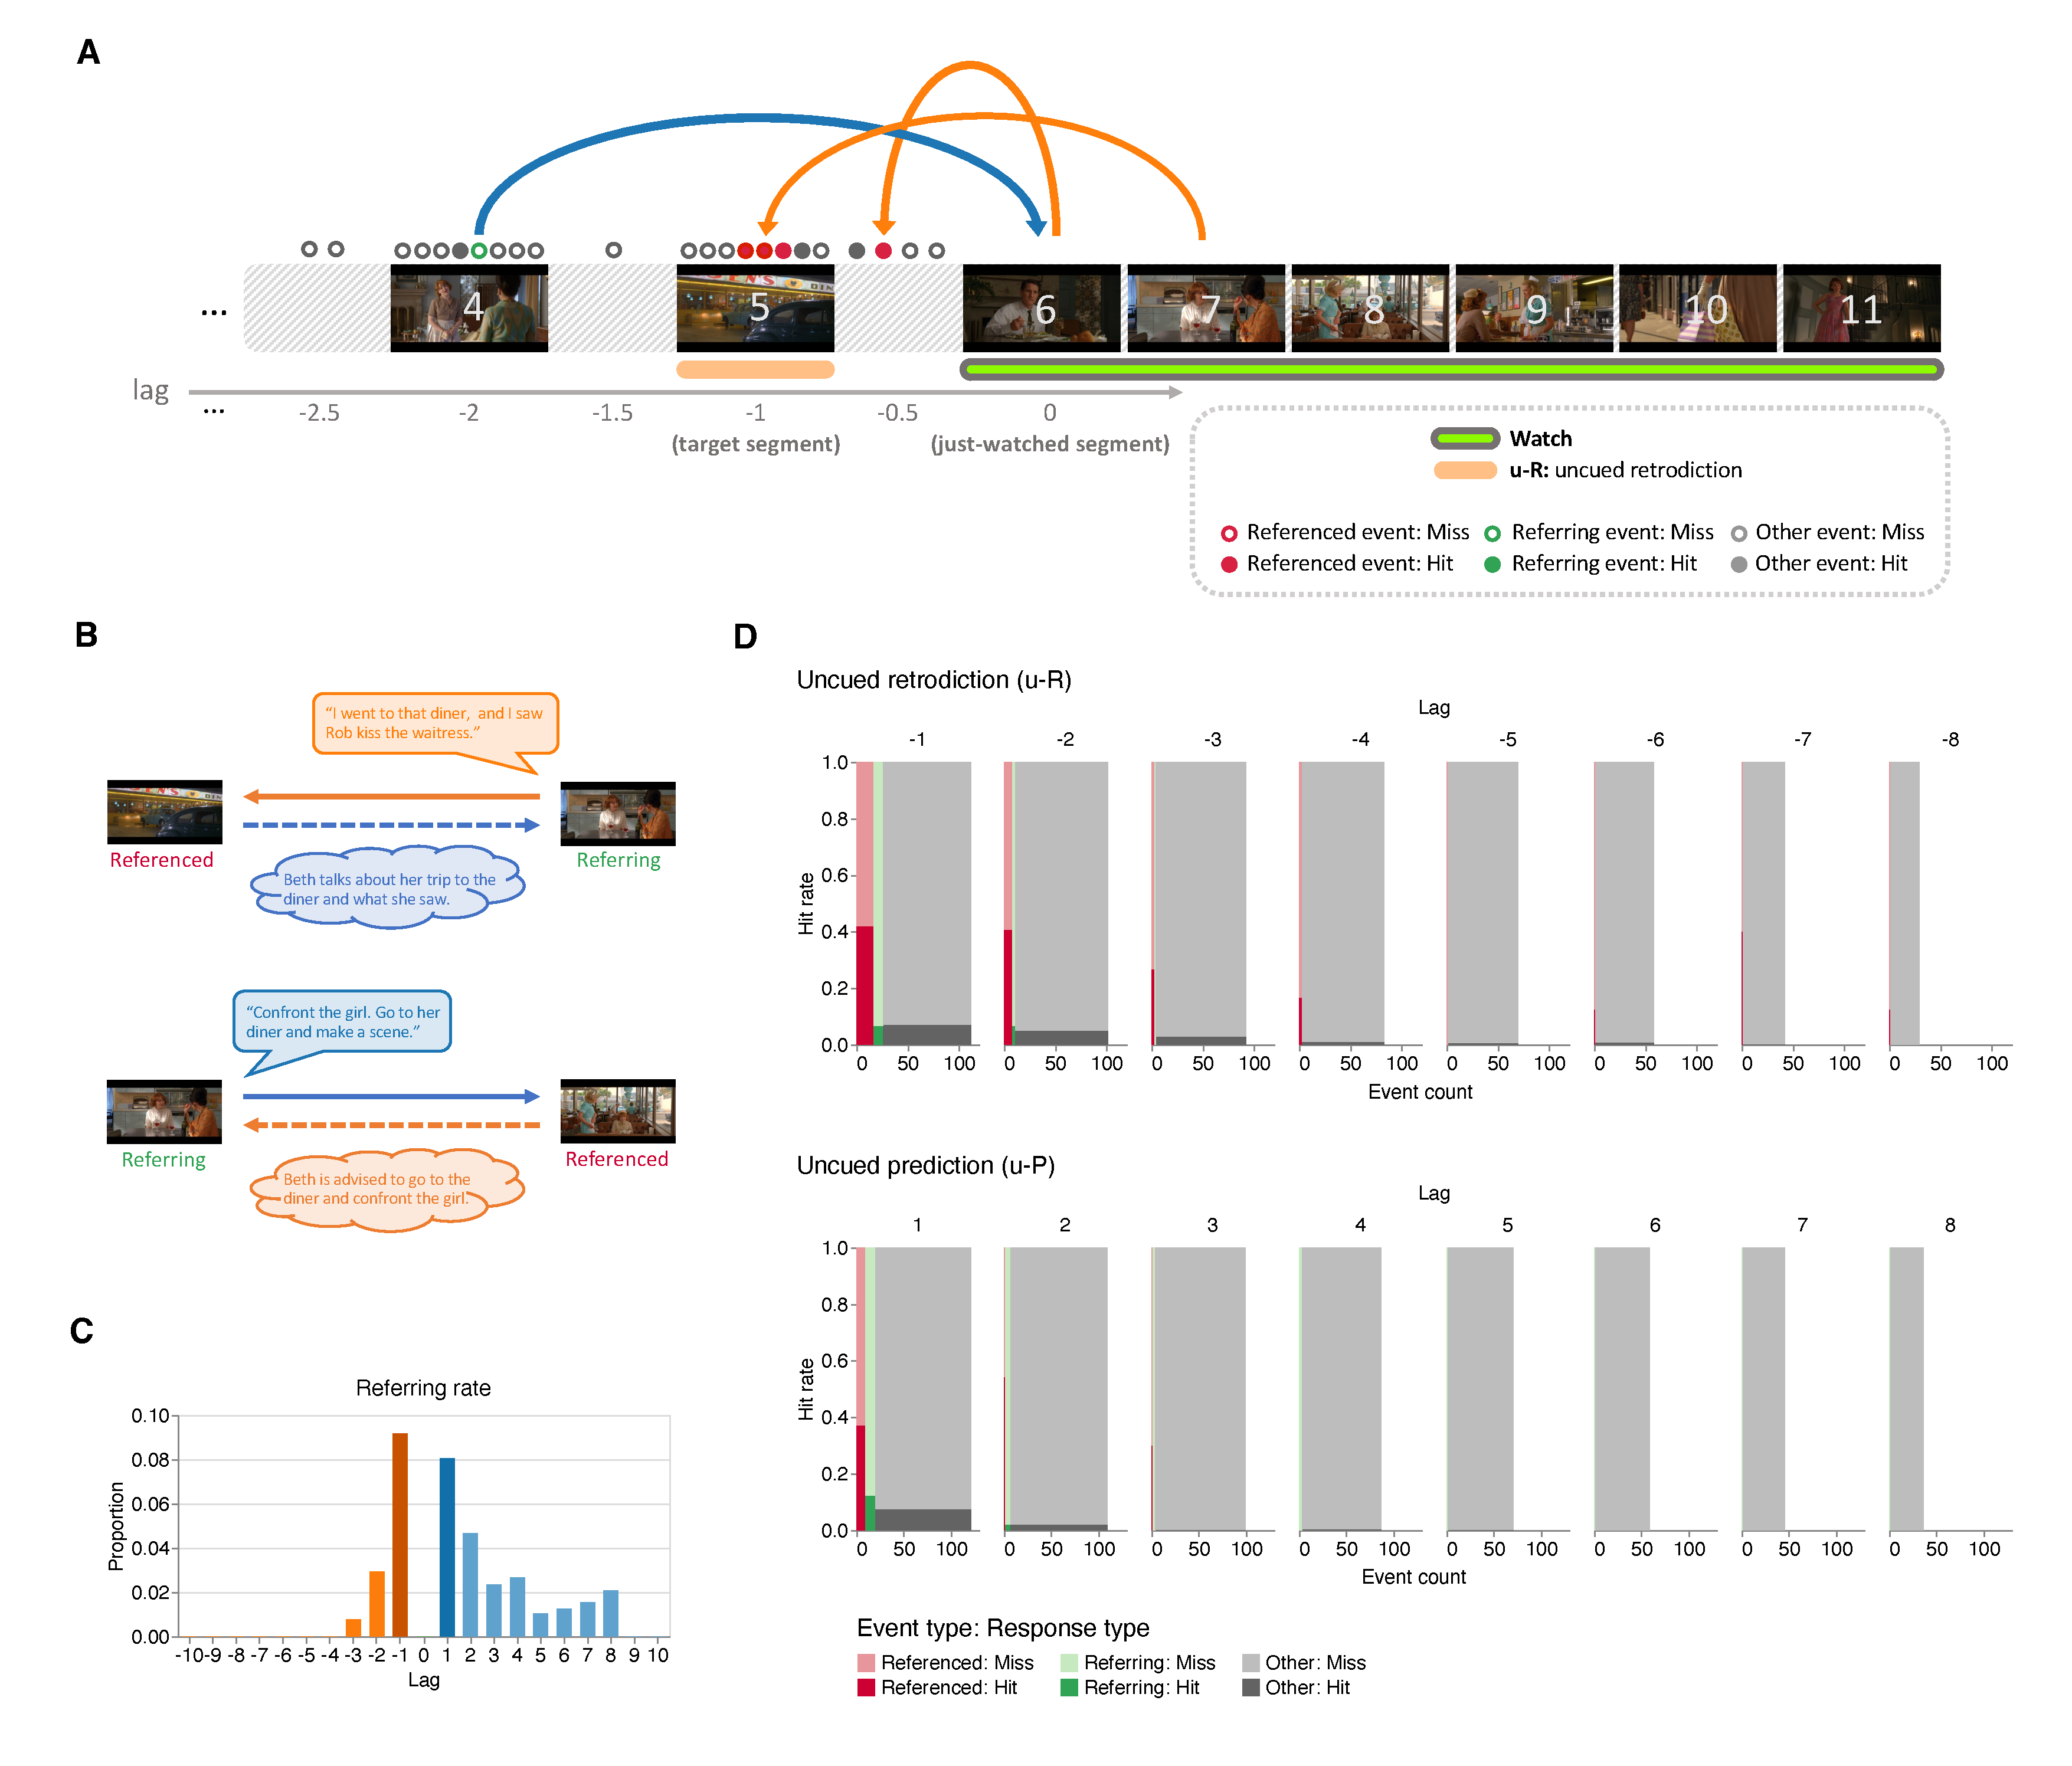
\includegraphics[width=\textwidth]{results5}

  \caption{\textbf{Referenced events are associated with higher hit rates, but
  referring events are not.} \textbf{A. Illustration of annotation approach.}
  We extended the annotation procedure depicted in Figure~\ref{fig:result3}A to
  also label which events in our main experiment's stimuli \textit{contained}
  references to events in other segments. \textbf{B. Referenced versus
  referring events.} During event $i$, when a character makes a reference to
  another event ($j$), we define $i$ as the \textit{referring} event and $j$ as
  the \textit{referenced} event. \textbf{C. Referring rate as a function of
  lag.} Across all possible just-watched segments (lag 0), the bar heights
  denote the across-segment mean proportions of events containing references to
  events in other past (orange, negative lags) or future (blue, positive lags)
  segments. The bar colors are described in the Figure~\ref{fig:result2}
  caption. \textbf{D. Hit rates and counts of referenced, referring, and other
  events.} As a function of temporal distance to the just-watched segment, the
  sub-panels display the numbers ($x$-axes) and hit rates ($y$-axes) of
  referenced (red), referring (green), and other (gray) events that
  participants hit (darker shading) or missed (lighter shading) in their uncued
  retrodictions (top sub-panel) and uncued predictions (bottom sub-panel). For
  a display of analogous results from our replication experiment see
  Figure~\referringReferenced.}

  \label{fig:result5}
\end{figure}

The preceding analyses show that when characters reference past or future
events, those referenced events, and other events that are temporally adjacent
to the referenced events, are more likely to be retrodicted and predicted. In
other words, referring to a past or future event in conversation leads to a
``boost'' in that event's hit rate. We wondered whether this boost was
bi-directional. In particular: when a character refers (during a
\textit{referring event}) to another event (i.e., the \textit{referenced
event}), does this boost only the referenced event's hit rate, or does the
referring event also receive a boost? We labeled each event as a ``referring
event,'' a ``referenced event,'' or a ``other event'' (i.e., not referring or
referenced; Fig.~\ref{fig:result5}A, B). We limited our analysis to references
to onscreen (explicit) events. Consistent with our analysis of the proportions
of referenced events (Fig.~\ref{fig:result3}B), the proportions of
\textit{referring} events exhibited a \textit{forward} temporal asymmetry
(Fig.~\ref{fig:result5}C). Controlling for absolute lag, we found that
referring events were associated with lower hit rates than referenced events in
our main experiment (uncued retrodiction: OR = 0.03, $Z = -4.81$, $p < 0.001$,
CI: 0.01 to 0.11; uncued prediction: OR = 0.04, $Z = -5.84$, $p < 0.001$, CI:
0.01 to 0.12; Fig.~\ref{fig:result5}D) and had no reliable differences in hit
rates compared with other events (uncued retrodiction: OR = 0.37, $Z = -1.46$,
$p = 0.15$, CI: 0.10 to 1.41; uncued prediction: OR = 2.16, $Z = 1.68$, $p =
0.09$, CI: 0.88 to 5.30). We also observed this phenomenon in our replication
experiment (referenced events, uncued retrodiction: OR = XXX, $Z = XXX$, $p =
XXX$, CI: XXX to XXX; referenced events, uncued prediction: OR = XXX, $Z =
XXX$, $p = XXX$, CI: XXX to XXX; other events, uncued retrodiction: OR = XXX,
$Z = XXX$, $p = XXX$, CI: XXX to XXX; other events, uncued prediction: OR =
XXX, $Z = XXX$, $p = XXX$, CI: XXX to XXX;Fig.~\referringReferenced). Taken
together, this indicates that only referenced events received a hit rate boost
(relative to other events), suggesting that the retrodictive and predictive
benefits of references are directed (i.e., asymmetric).

\begin{figure}[tp]
  \centering
  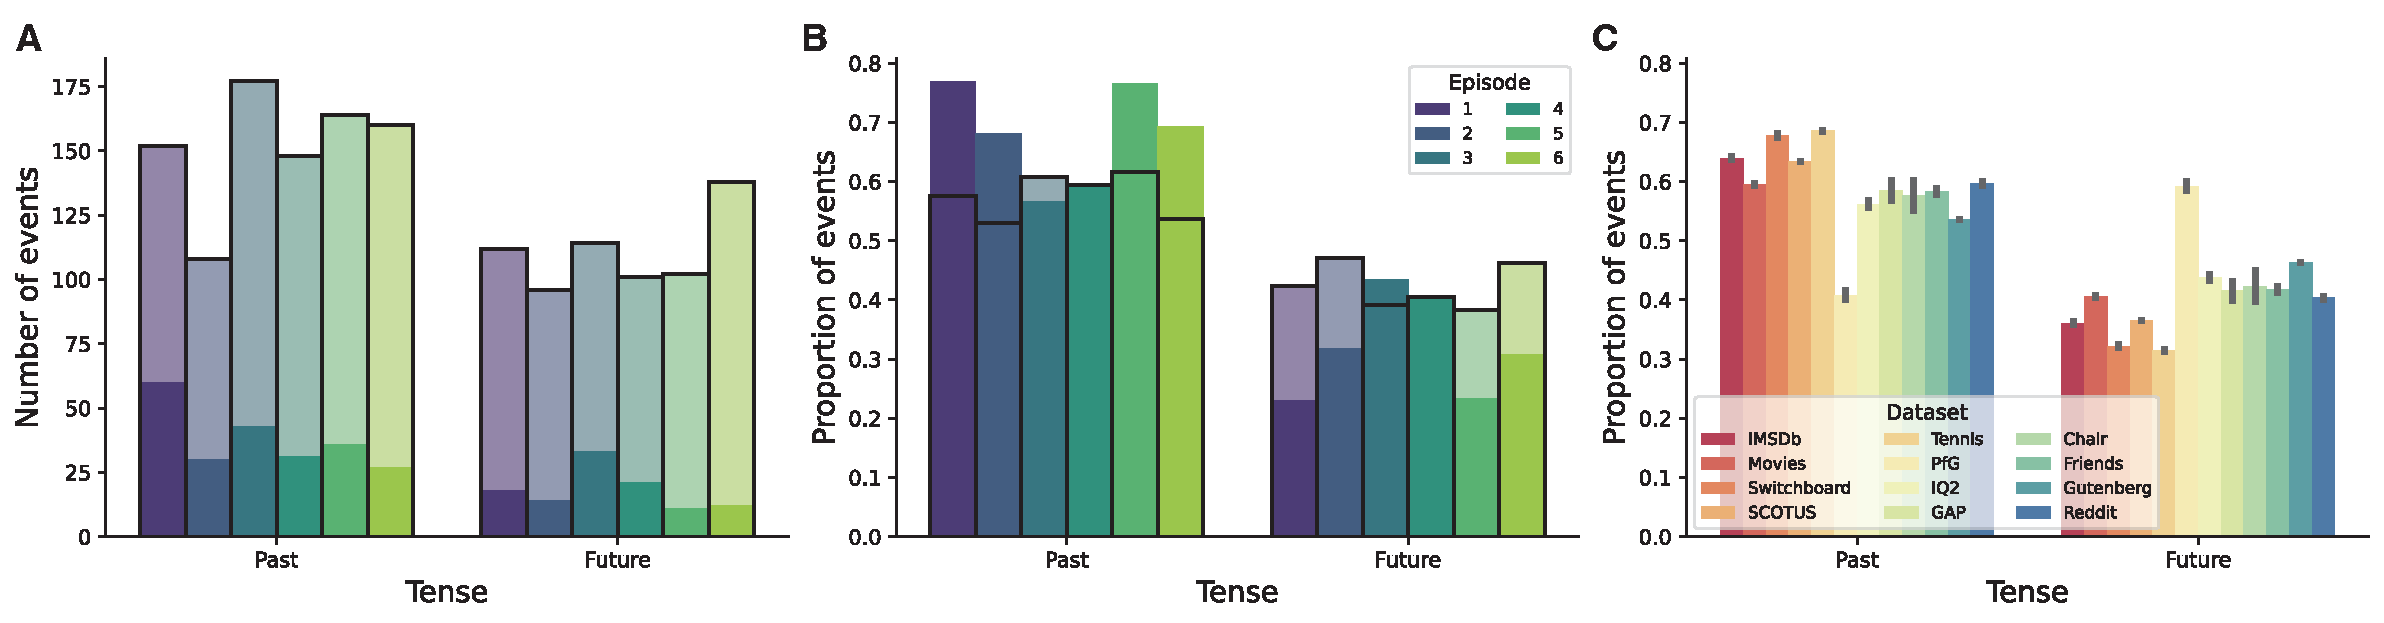
\includegraphics[width=\textwidth]{meta-analysis}

\caption{\textbf{Meta analysis.} We used natural language processing to
automatically identify references to past or future events across a variety of
sources. \textbf{A. Numbers of past and future events in \textit{The Chair},
Season 1, Episodes 1--6.} The bar heights indicate the raw numbers of manually
identified (lighter shading) and automatically identified (darker shading) past
and future events from each episode (color). We used Episode 1 from this series
as the stimulus in our replication experiment. \textbf{B. Proportions of past
and future events in \textit{The Chair}, Season 1, Episodes 1--6.} The Panel is
in the same format as Panel A, but here the bar heights have been divided by
the total numbers of past and future events (per episode). \textbf{C.
Proportions of past and future events in movies, television shows, and natural
conversations.} As in Panel B, the bar heights denote the proportions of past
and future events detected in each dataset (color). The datasets are described
in Table~\metaTable. Error bars denote bootstrap-estimated 95\% confidence
intervals.}
  
  \label{fig:meta-analysis}
\end{figure}

The above analyses show that characters in the television shows we used as
stimuli in our main experiment and replication experiment refer more often to
the past than to the future. This appears to bias participants' inferences
about the past and future. But how universal is this pattern? For example, were
the television shows we happened to select for our experiment representative of
television shows more generally? Or perhaps media created for entertainment
purposes tends to have a bias towards the past in order to keep the story
engaging and unpredictable. To better understand temporal biases in
conversations, we carried out a meta analysis using extracted conversation data
from several large datasets, comprising a total of over 440 million
conversations from over 17 million documents. The data comprised transcripts
from television shows and popular films, novels, and spoken and written
utterances from natural conversations. A summary of the data we analyzed may be
found in Table~\metaTable. As summarized in Figure~\ref{fig:meta-analysis}, we
used natural language processing to identify references to past or future
events in each conversation (also see \textit{Meta analysis of conversation
data}).

To validate our basic approach, we compared the numbers
(Fig.~\ref{fig:meta-analysis}A) and proportions (Fig.~\ref{fig:meta-analysis}B)
of automatically and manually identified references to past and future events,
across six episodes of the television show \textit{The Chair}. (The first
episode was used as the stimulus in our replication study.) In general, our
automated tagging procedure tended to overcount the numbers of references. From
manually inspecting hundreds of example tags, we believe this discrepancy
follows from which criteria were used to generate the tags. The manually
generated tags sought to identify references to specific events that occurred
or were implied to occur in other parts of the narrative. In contrast, as a
heuristic, we designed the automatic tagging procedure to identify uses of the
past or future \textit{tense} as a proxy for references to past or future
\textit{events}. We noticed that, a single conversation often contains multiple
references to a given (past or future) event. Whereas the manually generated
tags counted these as ``single'' references, our automated tagging procedure
had no means of differentiating between multiple references to the same event
versus references to different events. Nevertheless, this discrepancy did not
appear to bias the balance of the overall \textit{proportions} of past or
future references.

In all, across all of the datasets we examined in our meta analysis, we
identified a total of 36,008,500 references to past or future events. A total
of 19,464,741 (54.06\%) of these were references to past events, and the
remaining 16,543,759 (45.94\%) were references to future events. We also
computed the average proportions of references to past and future events across
documents within each individual dataset. Across the 12 datasets we examined
(Fig.~\ref{fig:meta-analysis}, Tab.~\metaTable), there were significantly more
references to the past than the to the future (mean $\pm$ standard deviation:
$58.99\% \pm 7.28\%$; $t(11) = 4.28, p = 0.0013$). This bias towards the past
also held for each dataset individually ($t$s $\geq 5.14$, $p$s $< 0.01$)
except for one dataset, ``Persuasion for Good,'' which comprised natural
conversations between pairs of Amazon Mechanical Turk workers wherein one
participant tried to convince the other participant to donate to a charity in
the future. In that dataset, references to the future were significantly more
common than references to the past ($t(11438) = -22.65, p < 0.001$). This
latter example provided a nice sanity check for verifying that our general
approach was not itself biased in favor of the past, e.g., even in
conversations that were actually biased towards the future. Taken together, the
results from our meta analysis indicate that people tend to refer to the past
more than they refer to the future, across a wide variety of situations
(including in both fictional and real conversations). Although (as in the
Persuasion for Good dataset) there may be specific exceptions to this bias, it
seems that a bias in favor of the past is a common element of many (and perhaps
even \textit{most}) human conversations.

\section*{Discussion}

We asked participants to watch sequences of movie segments from a
character-driven television drama and then either retrodict what had happened
prior to a just-watched segment, predict what would happen next, or recall what
they had just watched. We found that participants tended to more accurately and
more readily retrodict the unobserved past than predict the unobserved future.
We traced this temporal asymmetry to (a) characters' tendencies to refer to
past events more than future events in their ongoing conversations, and (b)
associations between temporally proximal events (Fig.~\ref{fig:discussion}).
Essentially, associations between temporally proximal events serve to enhance
asymmetries in inferences driven by conversational references (light orange and
blue bars in Fig.~\ref{fig:discussion}). Our findings show that other peoples'
psychological arrows of time can affect external observers' inferences about
the unobserved past and future.

\begin{figure}[tp]
  \centering
  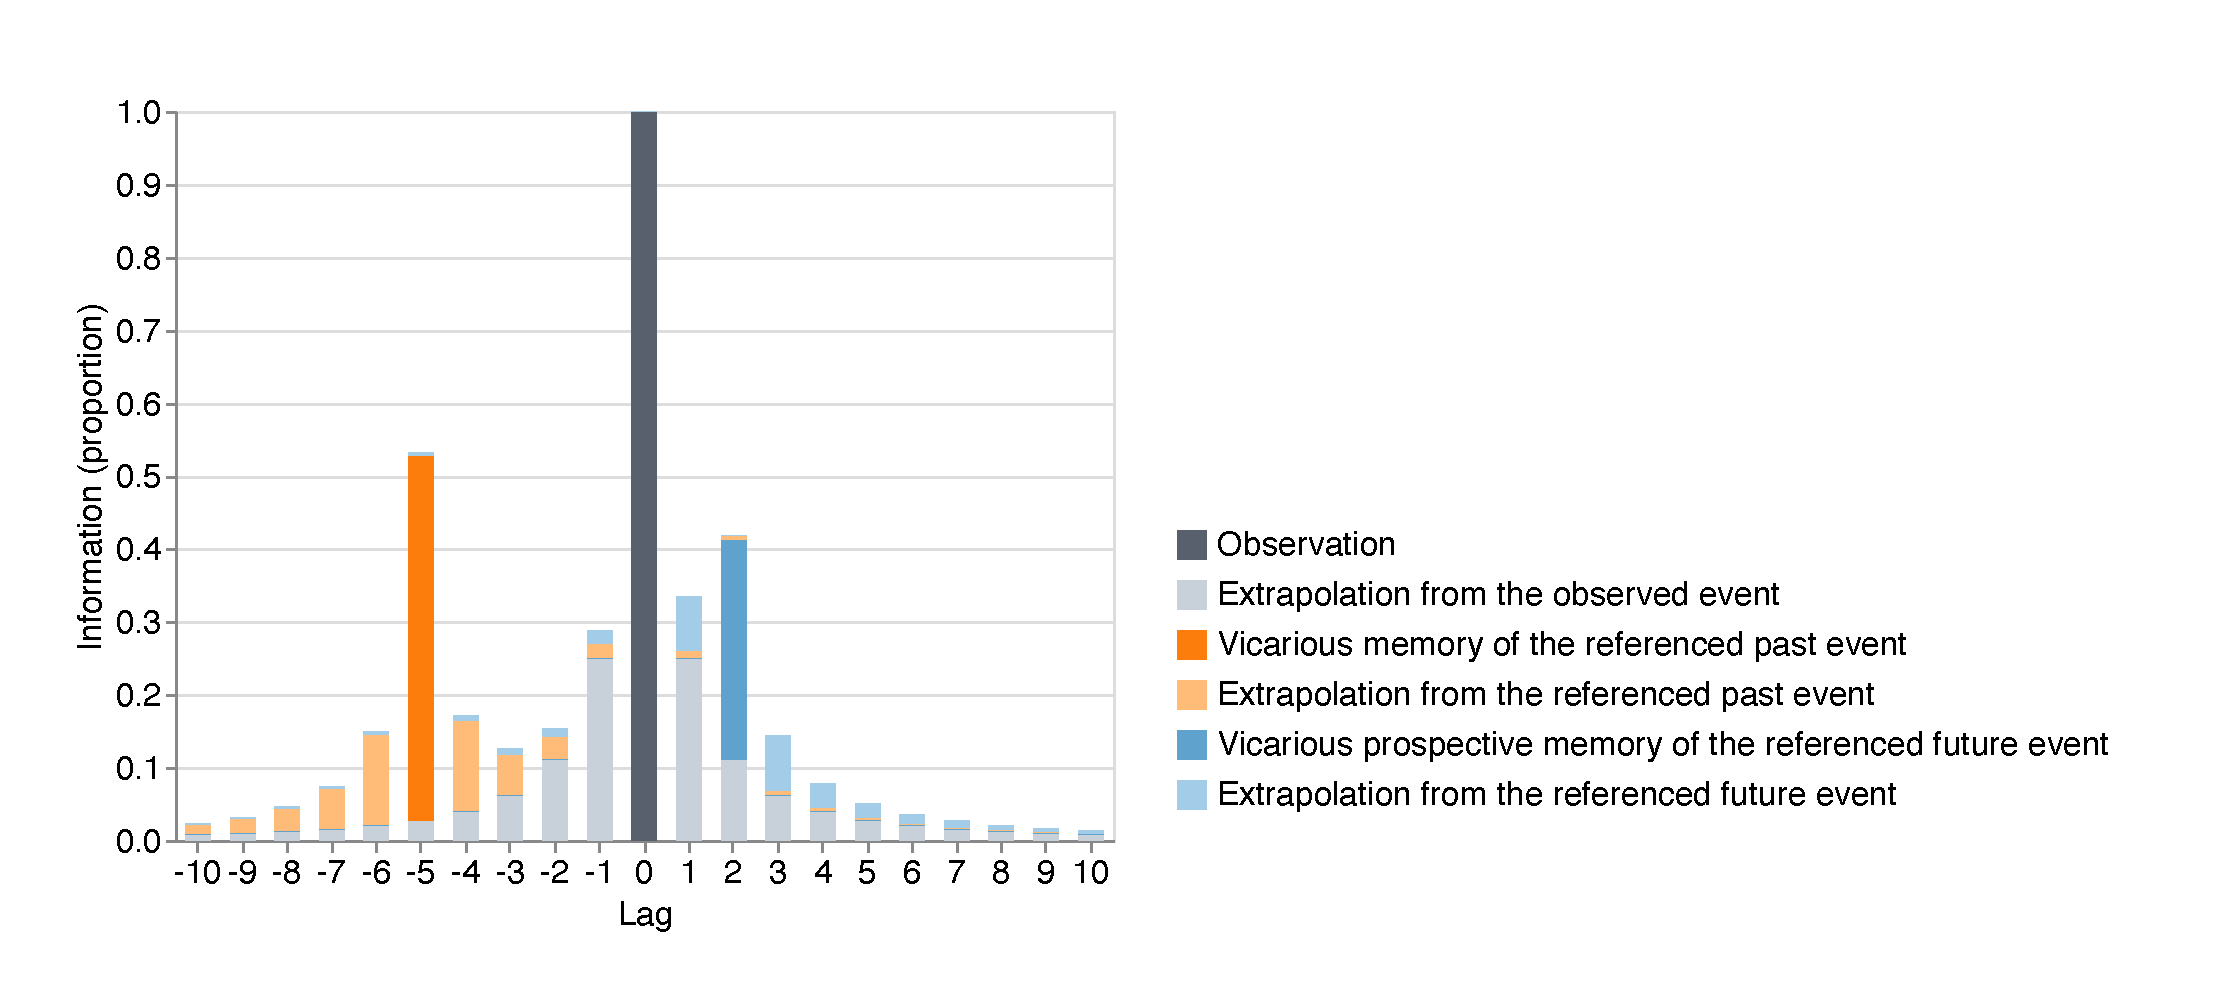
\includegraphics[width=\textwidth]{discussion}

  \caption{\textbf{How much information about the past and future can be
  inferred by observing the present?} By definition, let us say that the
  present moment (lag 0) contains all information about itself (dark gray).
  Given learned statistical regularities, one might extrapolate from the
  present moment into the past or future (light gray). As illustrated in this
  schematic, the information contained in the present about other moments in
  time falls off with absolute lag. This falloff is approximately
  time-symmetric. References in the present to past events (dark orange) or
  future events (dark blue) provide additional information about those
  referenced moments in time, beyond what could be inferred solely from
  statistical regularities. This additional information about those referenced
  moments can also be extrapolated to other moments that are temporally nearby
  to \textit{them} (light orange and blue).}

  \label{fig:discussion}
\end{figure}

When people communicate through language or other observable behaviors, they
can transmit their knowledge and memories to others~\citep{HirsEcht12,
MahrCsib18, Dess07, ZadbEtal17}. A consequence of this sharing across people is
that biases or limitations in one person's knowledge and memories may also be
transmitted to external observers. Although people \textit{can} communicate
their intentions and future plans (i.e., information about their future),
because people know \textit{more} about their pasts than their futures, the
knowledge transmitted to observers is inherently biased in favor of the
past~\citep[Fig.~\ref{fig:discussion}; ][]{DemiEtal18}. Since observers
leverage communicated knowledge to reconstruct the unobserved past and future,
this explains why observers' inferences about observed people's lives also
favor the past.

People's knowledge asymmetries are not always directly observable. For example,
in a conversation where someone talks exclusively about their future plans, a
passive observer might gain more insight into the speaker's unobserved future
than their unobserved past. However, because the speaker is also guided by
their own psychological arrow of time, the ``upper limit'' of knowledge about
their past is still higher than that of their future. Therefore, after
accounting for knowledge that \textit{could} be revealed through active
participation in the conversation, the seemingly future-biased conversation
masks an underlying knowledge asymmetry in favor of the past. This hypothesized
``unmasking'' effect of interaction implies that the influence of other
people's psychological arrows of time should be more robust when the receiver
is an active participant in the conversation. Other social dimensions, such as
trust, motivation or level of engagement, personal goals, and beliefs, might
serve to modulate the effective ``gain'' of the communication channel-- i.e.,
how much the speaker's knowledge influences the observer's knowledge.

In typical statistical sequences used in laboratory studies, there is no
temporal asymmetry, either theoretically~\citep{Cove94, BialEtal01,
ElliEtal09}, or empirically~\citep{JonePash07}. What makes narratives and
real-world event sequences time-asymmetric? Of course there are many
superficial differences between simple laboratory-manufactured sequences and
real-world experiences. As one example, real-world experiences often involve
other people who have their own memories and goals. At a deeper level, however,
are our subjective experiences essentially more complicated versions of
laboratory-manufactured sequences? Or are there fundamental differences? One
possibility is that real-life event sequences are not stationary~\citep[i.e.,
not in equilibrium,][]{Cove94}. For example, real-life events might start from
a special initial condition~\citep{Albe00, Feyn65, Cove94} and proceed through
a series of transitions from more-ordered to less-ordered states, thus
exhibiting an arrow time. When we retrodict, it is possible that we only
consider possible past events that are compatible with the highly-ordered
special initial state~\citep{Carr10, Carr16}. For example, when we see a broken
egg we might infer that the egg had been intact at some point in the past. But
it would be difficult to guess at what states or forms the broken egg might
take in the future~\citep{Carr10, Carr16}. In other words, the procession from
order to disorder might result in better retrodiction performance compared with
that of (implicitly less-restricted) prediction tasks. The special initial
state might also explain why we remember the past, but not the future. Some
recent work suggests that the psychological arrow of time might be explained by
a related concept in the statistical physics literature, termed the
``thermodynamic'' arrow of time~\citep{MlodBrun14, Rove22}. However, the
relation between the thermodynamic and psychological arrows of time is still
under debate~\citep{Golo21, HemmShen19}.

In our study, we explicitly designed participants' experiences such that both
the past and future were unobserved. How representative is this scenario of
everyday life? For example, we might try to speculate about the unobserved
future when making plans or goals, but when might we encounter situations where
the past is unobserved but still useful for us to speculate about? Real-life
events have long-range dependencies. In general, because the future depends on
what happened in the past, discovering or estimating information about the
unobserved past can help us form predictions about the future. We illustrate
this point in Figure~\ref{fig:discussion} by showing that the additional
information contributed by a referenced past event can also extend into the
future (light orange bars at lags $> 0$). This might explain why humans devote
substantial effort and resources to attempting to figure out what happened in
the unobserved past: history, anthropology, geology, detective and forensic
science, and other related fields are each primarily focused on understanding,
retrodicting, or reconstructing unobserved past events.


\section*{Methods}
\subsection*{Participants}

A total of 36 participants (25 female, mean age 21.47 years, range 19--50
years) were recruited from the Dartmouth College community. All participants
had self-reported normal or corrected-to-normal vision, hearing, and memory,
and had not watched any episodes of \textit{Why Women Kill} before the
experiment. Participants gave written consent to enroll in the study under a
protocol approved by the Committee for the Protection of Human Subjects at
Dartmouth College. Participants received course credit or monetary compensation
for their time. Two participants completed only the first half of the study and
one participant’s data from the second half of their testing session was lost
due to a technical error. All available data were used in the analyses.

\subsection*{Stimuli}

The stimulus used in the study were segments of the CBS television series
\textit{Why Women Kill} Season 1. The TV series contained three distinct
storylines depicting three women’s marital relationships. The three storylines,
which took place in the 1960s, 1980s, and 2019, were shown in an interleaved
fashion in the original episodes. The first 11 segments from the 1960s and
1980s storylines, across the first and second episodes, were used in our study.
Segments were divided based on major scene cuts, which primarily corresponded
to storyline shifts in the original episodes. The mean length of the segments
was 2.05 min (range 0.97--3.87 min). We chose this TV series based on its
strictly linear storytelling (within each storyline) and its realistic settings
where most events depicted everyday life. The plots were focused on the main
characters (Beth in storyline 1 and Simone in storyline 2), who were present in
all the segments in the corresponding storylines.

\subsection*{Task design and procedure}

Our experimental paradigm was divided across two testing sessions. In each
session, participants performed a sequence of tasks on segments from one
storyline (Fig.~\ref{fig:method}). For each storyline, there were four
different task sequences: two forward chronological order sequences and two
backward chronological order sequences. Participants completed one task
sequence in forward chronological order for one storyline, and one in backward
chronological order for the other storyline. The order of the two sessions
(forward chronological order sequence first or backward chronological order
sequence first), and the pairing of task sequences with storylines, were
counterbalanced across participants.

Tasks in each sequence alternated between watching, recall, and retrodiction or
prediction, with the specific order of tasks differing across the four
sequences. For example, in sequence A1, participants first watched segment 1,
followed by an immediate recall of segment 1. Then they predicted what would
happen in segment 2 (first uncued and then character-cued). Participants then
watched segment 3 and recalled segment 3. After that, participants guessed what
happened in segment 2 again, which we termed ``updated prediction''. Then they
watched segment 2, recalled segment 2, and so on as depicted in
Figure~\ref{fig:method}. This procedure was repeated to cover all possible
segments. We also note several edge cases at the start and end of the narrative
sequences. Since no segments precede the first segment, participants could
never make ``prediction'' responses with the first segment as their target. For
analogous reasons, participants never made ``retrodiction'' responses with the
last segment as their target. Another edge case occurred in task sequences B2
and A2 (Fig.~\ref{fig:method}). In the A1 and A2 sequences, participants
experience the narrative in the original (forward) order, predicting one
segment ahead along the way. In the B1 and B2 sequences, participants
experience the narrative in the reverse order, retrodicting one segment ahead
along the way. However, because A2 and B2 are offset from A1 and B2 by one
segment, the initial A2 responses are \textit{retro}dictions, and the initial
B2 responses are \textit{pre}dictions (i.e., they conflict with the temporal
directions of the remaining responses in those conditions). We therefore
excluded from our analysis those initial retrodiction responses from the A2
condition, and the initial prediction responses from the B2 condition.

Before watching each segment, participants were given the following task
instructions. After watching the video, participants were instructed to type
their responses (retrodiction, prediction, or recall) in 1--4 sentences.
Participants were also asked to specify the characters' names in their
responses, i.e., avoiding use of characters' pronouns. For the recall task, the
names of the characters in the recall segment were displayed, and participants
were asked to summarize the major plot points in the present tense. For the
retrodiction and prediction tasks, participants were instructed to retrodict or
predict the major plot points of the segment (also in the present tense), as
though they had watched the segment and were writing a plot synopsis. They were
also instructed to avoid speculation words (e.g., ``I \textit{think} Beth
will...''). For the uncued retrodiction and prediction tasks, participants made
retrodictions or predictions without any cues provided, so they had to guess
which of the characters would be present in the segment. For character-cued
retrodictions and predictions, the characters in the target segment were
revealed on the screen, alongside participants’ previous responses.
Participants were instructed to include or incorporate those characters into
their character-cued responses, if their previous responses did not contain all
the characters provided. They were also told that the characters were not
necessarily listed in their order of appearance in the segment, and that only
the main characters would be given. Also, the characters given did not
necessarily interact with each other in that segment, and they could appear in
successive events in that segment. If participants’ previous responses included
all the characters given, then they could directly proceed to the next task
without updating their responses. For all of the prediction and retrodiction
tasks, participants were instructed to provide at least one response, but they
were given the opportunity enter up to three responses if they felt that
multiple possibilities were more or less equally likely. Each response
(including recall) was followed by a confidence rating on a 1--5 point scale.
However, these confidence data were not analyzed in the present study.

Before their first testing session, participants were given a practice session,
where they watched the first segment of storyline 3 followed by a recall trial,
an uncued prediction trial, and a character-cued prediction trial.
Participants' responses were checked by the experimenter to ensure compliance
with the instructions. To provide participants with sufficient background
information about the storyline (especially for the backward chronological
sequences), at the beginning of each session, participants were shown the time,
location, and the main characters (with pictures) of the storyline. The first
session was approximately 1.5~h long and the second session was approximately
1~h long. We allowed participants, at their own discretion and convenience, to
sign up for two consecutive testing time-slots (i.e., with their testing
sessions occurring in immediate succession), or for testing sessions on two
different days. The mean inter-session interval was 0.73 days (range: 0--4
days). The experiment was conducted in a sound- and light-attenuated testing
room. Videos were displayed using a 27-inch iMac desktop computer (resolution:
$5120 \times 2880$) and sound was presented using the iMac’s built-in speakers.
The experiment was implemented using jsPsych~\citep{deLe15} and
JATOS~\citep{LangEtal15}.

\subsection*{Video annotation}

Events in the first 11 segments of the two storylines were identified by the
first author (X.X.), corresponding to major plot points (total: 117; mean: 5.32
per segment; range 3--9). Additionally, 74 offscreen events were identified. Of
these 74 offscreen events, 43 events were identified from references in
conversations during onscreen events. Another 16 events were identified based
on characters’ implied movements and travels. For example, if in segment 1
character A was in place A and in segment 2 she was in place B, then the
transit from place A to B for character A would be identified as an offscreen
event. The remaining 15 offscreen events were identified based on logical
inferences. For example, if a photograph was shown in an onscreen event (but
not the act of the photograph being taken), then the action that someone took
the photograph would be identified as an offscreen event. Offscreen events
always occurred between two contiguous segments, or before the first segment.
The purpose of identifying offscreen events was to match participants’
responses to video events; thus our identification of these offscreen events
was not intended to be exhaustive.

\subsection*{Response analyses}

Participants' retrodiction, prediction, and recall responses were minimally
processed to correct obvious typos (e.g., in characters’ names) and remove
speculation descriptions (e.g., ``I predict that...''). All responses were
manually coded and matched to events from the video annotations. Retrodiction
and prediction responses were coded by two coders (X.X. and Z.Z.). Recall
responses were coded by one coder (X.X.). While most responses were clearly
identifiable as either matching specific storyline events or as not matching
any storyline events, several ambiguous cases arose. First, some responses
combined or summarized over several (distinct) storyline events. Second, some
responses lacked any specific detail (e.g., ``character A and B talk'' without
describing the specific topic(s) of conversation or providing other relevant
details). Based on participants' responses, in addition to the original 117
onscreen events and 74 offscreen events, we added 25 new events (23 onscreen, 2
offscreen) that either summarized across several events or partially matched
the annotated events. Whereas the original events were each assigned a value of
one point, we assigned these additional events a half point. This point system
enabled us to directly match events in participants' responses to the annotated
events. In our analyses of retrodictions, predictions, and recalls, we added up
the number of points earned for each response to estimate participants' event
hit rates.

We coded only the first retrodiction or prediction response in each trial. For
these responses, we also only considered storyline events that were in the same
temporal direction as the target segment. For example, if a participant was
asked to retrodict what happened in segment $n$, only events from segments
$1...n$ were considered in our analysis. When coding recall responses, we
considered only events from the target segment.

An additional ambiguous case arose in one participant's responses pertaining to
segment 12, storyline 2, whereby the participant correctly identified an
onscreen event that had not been included in our original annotations. To
account for this participant's response, we retroactively added that event to
our annotations of that segment. We also identified and counted unmatched
events in participants' responses (i.e., events that did not match any
annotated events). Cases where the two coders' independent scoring disagreed
were resolved through discussions between the two coders.

To estimate the semantic similarities between pairs of responses, we first
transformed each response into a 512-dimensional vector (embedding) using the
Universal Sentence Encoder~\citep[Transformer USE, ][]{CerEtal18}. We defined
\textit{similarity} as the cosine of the angle formed by the responses'
vectors. Following~\cite{HeusEtal21}, we defined the \textit{precision} of
participants' responses as the median similarity between that response's vector
and the embedding vectors for all other participants' recalls of the target
segment. We defined the \textit{convergence} of a given response as the mean
similarity between that response's vector and all other participants' responses
to the corresponding segment, in the same condition. To compute these median or
mean similarities we first applied the Fisher $z$-transformation to the
similarity values, then took the median or mean of the $z$-transformed
similarities, and finally applied the inverse $z$-transformation to obtain the
precision or convergence score.

To test the validity and reliability of the USE embeddings, we performed a
classification analysis of recall responses using a leave-one-out approach. For
each recall response, we calculated its semantic similarity with all other
recall responses for the same storyline. We took the segment with the highest
median semantic similarity (to the recall response) as the ``predicted''
segment. Across all responses, the predicted segments matched the true recalled
segments' labels 98.6\% of the time (1088 out of 1103 predictions; chance
level: 9\%).

\subsection*{Reference coding}

Two coders (X.X. and Z.Z.) identified character dialogues in the narrative that
referred to past events or future (onscreen or offscreen) events. Only
references to events that occurred in a different segment were included in this
tagging procedure. For each reference, the source (referring) segment and the
referred event number were recorded. A total of 82 references were identified.
Of these, 30 referred to onscreen events and 52 referred to offscreen events.
For these referenced events, their corresponding summary events or partial
events were also labelled as referenced. In instances where the coders
disagreed about a given tag, disagreements were resolved through discussions
between the two coders. In our analyses, each storyline event was coded
according to whether or not it had been referenced in the segment(s) that the
participant had viewed thus far in the experiment.

In principle, a given event could receive multiple labels. For example, during
event $A$, a character might speak about another event, $B$, during which a
reference to a third event ($C$) was made. In this scenario, event $B$ could be
both a ``referring event'' ($B \rightarrow C$) \textit{and} a referenced event
($A \rightarrow B$). In practice, however, this scenario was quite rare,
accounting for only one out of a total of 30 onscreen events.

\subsection*{Statistical analysis}

We used (generalized) linear mixed models to analyze the hit rates and numbers
of events retrodicted, predicted, and recalled, as well as the precisions and
convergences of participants' responses. Our models were implemented in
\texttt{R} using the \texttt{afex} package. We carried out comparisons or
contrasts, and extracted $p$-values, using the \texttt{emmeans} package.
Participants and stimuli (e.g., segment identity) were modeled as crossed
random effects (as specified below). Random effects were selected as the
maximal structure that allowed model convergence. All of our statistical tests
were two-sided.

For our tests of the target event hit rates across four \texttt{levels}
(uncued, character-cued, updated, and recall; Fig.~\ref{fig:result1}B), we fit
a generalized linear mixed model with a binomial link function:
\begin{lstlisting}[language=R]
  cbind(thp, ttp - thp) ~ direction * level * seg_cnt * storyline +
(direction * level | target) +
(direction * level * seg_cnt | subject)
\end{lstlisting}
where \texttt{thp} was the number of points hit for the target segment,
\texttt{ttp} was the total number of points for the target segment (from its
annotations), \texttt{direction} was either retrodiction or prediction,
\texttt{level} had four levels (uncued, character-cued, updated, and recall),
\texttt{seg\_cnt} represented the number of segments in the storyline that had
been watched (1--10, centered), \texttt{storyline} had two levels (1 or 2), and
\texttt{target} had 22 levels according to the identity of the target segment.
For our tests of precision and convergence (Fig.~\ref{fig:result1}C, D), we fit
linear mixed models using the same formula. To test the effect of
\texttt{direction} (retrodiction or prediction) on target event hit rates,
precision, and convergence, we fit a (generalized) linear mixed model
separately for each of the three levels (uncued, character-cued, and recall).

For our tests comparing the numbers of hits for different types of events
(Fig.~\ref{fig:result2}B), we fit generalized linear mixed models using the
same formula, but with a Poisson link function. For these models, we manually
doubled the point counts to ensure that half points were mapped onto integers,
ensuring compatibility with the Poisson link function.

For our analyses of the numbers of events hit, controlling for lag
(Fig.~\ref{fig:result2}C), we fit a generalized linear mixed model with a
Poisson link function:
\begin{lstlisting}[language=R]
  hp_lag ~ direction * full_stp * lag * storyline +
  (direction | base_seg) + (1 | base_seg_pair) +
  (direction * full_stp * lag * storyline | subject)
  \end{lstlisting}
where \texttt{hp\_lag} is the number of ``points'' earned (for each lag) in
each trial (we manually doubled the point counts to ensure that half points
were mapped onto integers, for compatibility with the Poisson link function),
\texttt{full\_stp} denoted whether the given events (of the given lag) were
onscreen (i.e., full step) or offscreen (i.e., half step), \texttt{lag} denotes
the (centered) absolute lag, \texttt{base\_seg} denotes the identity of the
just-watched segment (22 levels), and \texttt{base\_seg\_pair} denotes the
pairing of the just-watched segment and the segment at each lag (440 levels).

For our analyses of the proportions of events hit for referenced versus
unreferenced events (Fig.~\ref{fig:result3}D, E), we fit a generalized linear
model with a binomial link function:
\begin{lstlisting}[language=R]
  cbind(hp_lag, tp_lag - hp_lag) ~ direction * reference * full_stp +
  lag + (direction | base_seg) +
  (1 | base_seg_pair) +
  (direction * reference * full_stp + lag | subject)
\end{lstlisting}
where \texttt{hp\_lag} denotes the number of earned hit points for each
reference type (referenced or unreferenced) at each lag, \texttt{tp\_lag}
denotes the total number of possible hit points for each reference type at each
lag, and the other variables adhered to the same notation used in the above
formulas.

For our tests of the proportions of events hit for all three reference types
(referenced, reference-adjacent, and remaining: Fig.~\ref{fig:result4}D, E; or
referenced, referring, and other: Fig.~\ref{fig:result5}D), we fit a
generalized linear mixed model using the same formula as above, but with three
(rather than two) \texttt{reference} levels.

\section*{Code and data availability}

All of the code and data generated for the current manuscript are available
online at:

https://github.com/ContextLab/prediction-retrodiction-paper

% \bibliographystyle{apa}
\bibliography{cdl}

\section*{Acknowledgements}

We thank Luke Chang, Yi Fang, Paxton Fitzpatrick, Caroline Lee, Meghan Meyer,
Lucy Owen, and Kirsten Ziman for feedback and scientific discussions. Our work
was supported in part by NSF CAREER Award Number 2145172 to J.R.M. The content
is solely the responsibility of the authors and does not necessarily represent
the official views of our supporting organizations. The funders had no role in
study design, data collection and analysis, decision to publish, or preparation
of the manuscript.

\section*{Author contributions}

Conceptualization: X.X. and J.R.M.; Methodology: X.X. and J.R.M.; Software:
X.X.; Analysis: X.X., Z.Z., X.Z., and J.R.M.; Writing, Reviewing, and Editing:
X.X., Z.Z., X.Z., and J.R.M.; Supervision: J.R.M.

\section*{Competing interests}

The authors declare no competing interests.

\end{document} 